\documentclass[12pt, twoside]{report}
\usepackage[a4paper, top=2.0cm, bottom=2.0cm, left=2.5cm, right=2.5cm]{geometry}

\usepackage[MeX]{polski} 
\usepackage[T1]{fontenc}
\usepackage[utf8]{inputenc}
\usepackage{times}
\usepackage{color}
\usepackage{comment}
\usepackage{indentfirst}
\usepackage{graphicx}
\usepackage{mathptmx}
\usepackage{amsmath}
\usepackage{tikz}
\usepackage{hyperref}
\usepackage[final]{pdfpages}
\usepackage{afterpage}
\usepackage{titlesec}
\usepackage{microtype}
\usepackage{enumitem}
\usepackage{caption}
\usepackage{subcaption}
\usepackage{listings}
\usepackage{chngcntr}

\ProvidesPackage{java}

\graphicspath{{images/}}
\definecolor{dkgreen}{rgb}{0,0.6,0}
\definecolor{gray}{rgb}{0.5,0.5,0.5}
\definecolor{mauve}{rgb}{0.58,0,0.82}
\definecolor{gray}{rgb}{0.4,0.4,0.4}
\definecolor{darkblue}{rgb}{0.0,0.0,0.6}
\definecolor{lightblue}{rgb}{0.0,0.0,0.9}
\definecolor{cyan}{rgb}{0.0,0.6,0.6}
\definecolor{darkred}{rgb}{0.6,0.0,0.0}
\colorlet{punct}{red!60!black}
\definecolor{background}{HTML}{EEEEEE}
\definecolor{delim}{RGB}{20,105,176}
\colorlet{numb}{magenta!60!black}
\counterwithin{figure}{section}

\setlength{\parindent}{4em}
\titlespacing{\chapter}{0pt}{-35px}{5px}
\titlespacing*{\subsection}{0pt}{0px}{0px}
\titlespacing*{\subsubsection}{0pt}{0px}{0px}
\titlespacing*{\section}{0pt}{0px}{0px}
       
\titleformat{\chapter}[block]
       {\normalfont\huge\bfseries}{ \thechapter}{15pt}{\Huge}
       
\lstset{
  basicstyle=\ttfamily\footnotesize,
  columns=fullflexible,
  showstringspaces=false,
  numbers=left,                   % where to put the line-numbers
  numberstyle=\tiny\color{gray},  % the style that is used for the line-numbers
  stepnumber=1,
  numbersep=5pt,                  % how far the line-numbers are from the code
  backgroundcolor=\color{white},      % choose the background color. You must add \usepackage{color}
  showspaces=false,               % show spaces adding particular underscores
  showstringspaces=false,         % underline spaces within strings
  showtabs=false,                 % show tabs within strings adding particular underscores
  frame=single,                   % adds a frame around the code
  rulecolor=\color{black},        % if not set, the frame-color may be changed on line-breaks within not-black text (e.g. commens (green here))
  tabsize=2,                      % sets default tabsize to 2 spaces
  captionpos=b,                   % sets the caption-position to bottom
  breaklines=true,                % sets automatic line breaking
  breakatwhitespace=false,        % sets if automatic breaks should only happen at whitespace
  title=\lstname,                   % show the filename of files included with \lstinputlisting;
                                  % also try caption instead of title  
  commentstyle=\color{gray}\upshape
}

\lstdefinelanguage{XML}
{
  morestring=[s][\color{mauve}]{"}{"},
  morestring=[s][\color{black}]{>}{<},
  morecomment=[s]{<?}{?>},
  morecomment=[s][\color{dkgreen}]{<!--}{-->},
  stringstyle=\color{black},
  identifierstyle=\color{lightblue},
  keywordstyle=\color{red},
  morekeywords={xmlns,xsi,noNamespaceSchemaLocation,type,id,x,y,source,target,version,tool,transRef,roleRef,objective,eventually}% list your attributes here
}
\lstdefinelanguage{java}{%
  % Basic settings
  tabsize=4,
  %frame=single,
  showstringspaces=false,
  mathescape=true,
  breaklines=true,
  numbers=left,
  % Keywords, strings, and comments
  keywords={%
    abstract, continue, for, new, switch, assert, default, goto, package,
    synchronized, boolean, do, if, private, this, break, double, implements,
    protected, throw, byte, else, import, public, throws, case, enum,
    instanceof, return, transient, catch, extends, int, short, try, char,
    final, interface, static, void, class, finally, long, strictfp, volatile,
    const, float, native, super, while
  },
  keywords=[2]{%
  },
  morestring=[b]",
  morestring=[b]',
  morecomment=[l]{//},
  morecomment=[s]{/*}{*/},
  % Colors and style
  %backgroundcolor=\color{BackgroundYellow},
  keywordstyle=\color{blue},
  keywordstyle=[2]\color{DarkOrchid},
  commentstyle=\color{ForestGreen},
  stringstyle=\color{darkred},
  numberstyle=\color{gray}
}
\lstdefinelanguage{JavaScript}{
  keywords={typeof, new, true, false, catch, function, return, null, catch, switch, var, if, in, while, do, else, case, break},
  keywordstyle=\color{blue}\bfseries,
  ndkeywords={class, export, boolean, throw, implements, import, this},
  ndkeywordstyle=\color{darkgray}\bfseries,
  identifierstyle=\color{black},
  sensitive=false,
  comment=[l]{//},
  morecomment=[s]{/*}{*/},
  commentstyle=\color{purple}\ttfamily,
  stringstyle=\color{red}\ttfamily,
  morestring=[b]',
  morestring=[b]"
}
\lstdefinelanguage{HTML5}{
    sensitive=true,
    keywords={%
    % JavaScript
    typeof, new, true, false, catch, function, return, null, catch, switch, var, if, in, while, do, else, case, break,
    % HTML
    html, title, meta, style, head, body, script, canvas,
    % CSS
    border:, transform:, -moz-transform:, transition-duration:, transition-property:,
    transition-timing-function:
    },
    % http://texblog.org/tag/otherkeywords/
    otherkeywords={<, >, \/},   
    ndkeywords={class, export, boolean, throw, implements, import, this},   
    comment=[l]{//},
    % morecomment=[s][keywordstyle]{<}{>},  
    morecomment=[s]{/*}{*/},
    morecomment=[s]{<!}{>},
    morestring=[b]',
    morestring=[b]",    
    alsoletter={-},
    alsodigit={:}
}

\lstdefinelanguage{JSON}{%
    numbers=left,
    showstringspaces=true,
    breaklines=true,
    frame=single,
    literate=
     *{0}{{{\color{numb}0}}}{1}
      {1}{{{\color{numb}1}}}{1}
      {2}{{{\color{numb}2}}}{1}
      {3}{{{\color{numb}3}}}{1}
      {4}{{{\color{numb}4}}}{1}
      {5}{{{\color{numb}5}}}{1}
      {6}{{{\color{numb}6}}}{1}
      {7}{{{\color{numb}7}}}{1}
      {8}{{{\color{numb}8}}}{1}
      {9}{{{\color{numb}9}}}{1}
      {:}{{{\color{punct}{:}}}}{1}
      {,}{{{\color{punct}{,}}}}{1}
      {\{}{{{\color{delim}{\{}}}}{1}
      {\}}{{{\color{delim}{\}}}}}{1}
      {[}{{{\color{delim}{[}}}}{1}
      {]}{{{\color{delim}{]}}}}{1},
}

\linespread{1.5}

\newcommand\tab[1][0.5cm]{\hspace*{#1}}



\hypersetup{
    colorlinks,
    citecolor=black,
    filecolor=black,
    linkcolor=black,
    urlcolor=black
}

\newcommand\blankpage{%
	\null
    \thispagestyle{empty}%
    \newpage}

\pdfinfo{
   /Author (Krzysztof Dragan)
   /Title  (Aplikacja internetowa do wyszukiwania połączeń lotniczych)
   /CreationDate (\today)
   /Keywords (Praca;dyplomowa;inzynierska;modyfikacja;stfc)
}

 
% ------------ Początek dokumentu ------------
\begin{document}
\counterwithin{lstlisting}{section}
% Zmienia numerację listingu na numer aktualnego rozdziału
% --------------------------------------------
% -------------- Strona tyłułowa -------------
\afterpage{\blankpage}
\begin{titlepage}
	\centering
		
	{\fontsize{16pt}{12pt}\selectfont
		\MakeUppercase{\textls[150]{Politechnika Świętokrzyska}}\\ 
		Wydział Elektrotechniki, Automatyki i Informatyki \par}
		
	\vspace{0.1cm}
	\hrule
	\vspace{2.5cm}
		
	{\fontsize{14pt}{12pt}\selectfont
		\scshape\textbf{Krzysztof Dragan}}\\
	Numer albumu: 083524
	\\
	\vfill
	{\fontsize{20pt}{12pt}\selectfont
		\bfseries Aplikacja internetowa\\ do wyszukiwania połączeń lotniczych\par}
	\vspace{1cm}
	{\fontsize{14pt}{12pt}\selectfont
		Praca dyplomowa inżynierska\\
		na kierunku Informatyka\\ \par}
	\vspace{7cm}
	\hfill	Opiekun pracy dyplomowej:\par
	\hfill dr inż. Arkadiusz \textsc{Chrobot}\par
	\hfill Katedra Systemów Informatycznych
	\vfill
	Kielce \the\year \par
\end{titlepage}

% --------------------------------------------
% ------------------ Zadanie -----------------
\afterpage{\blankpage}
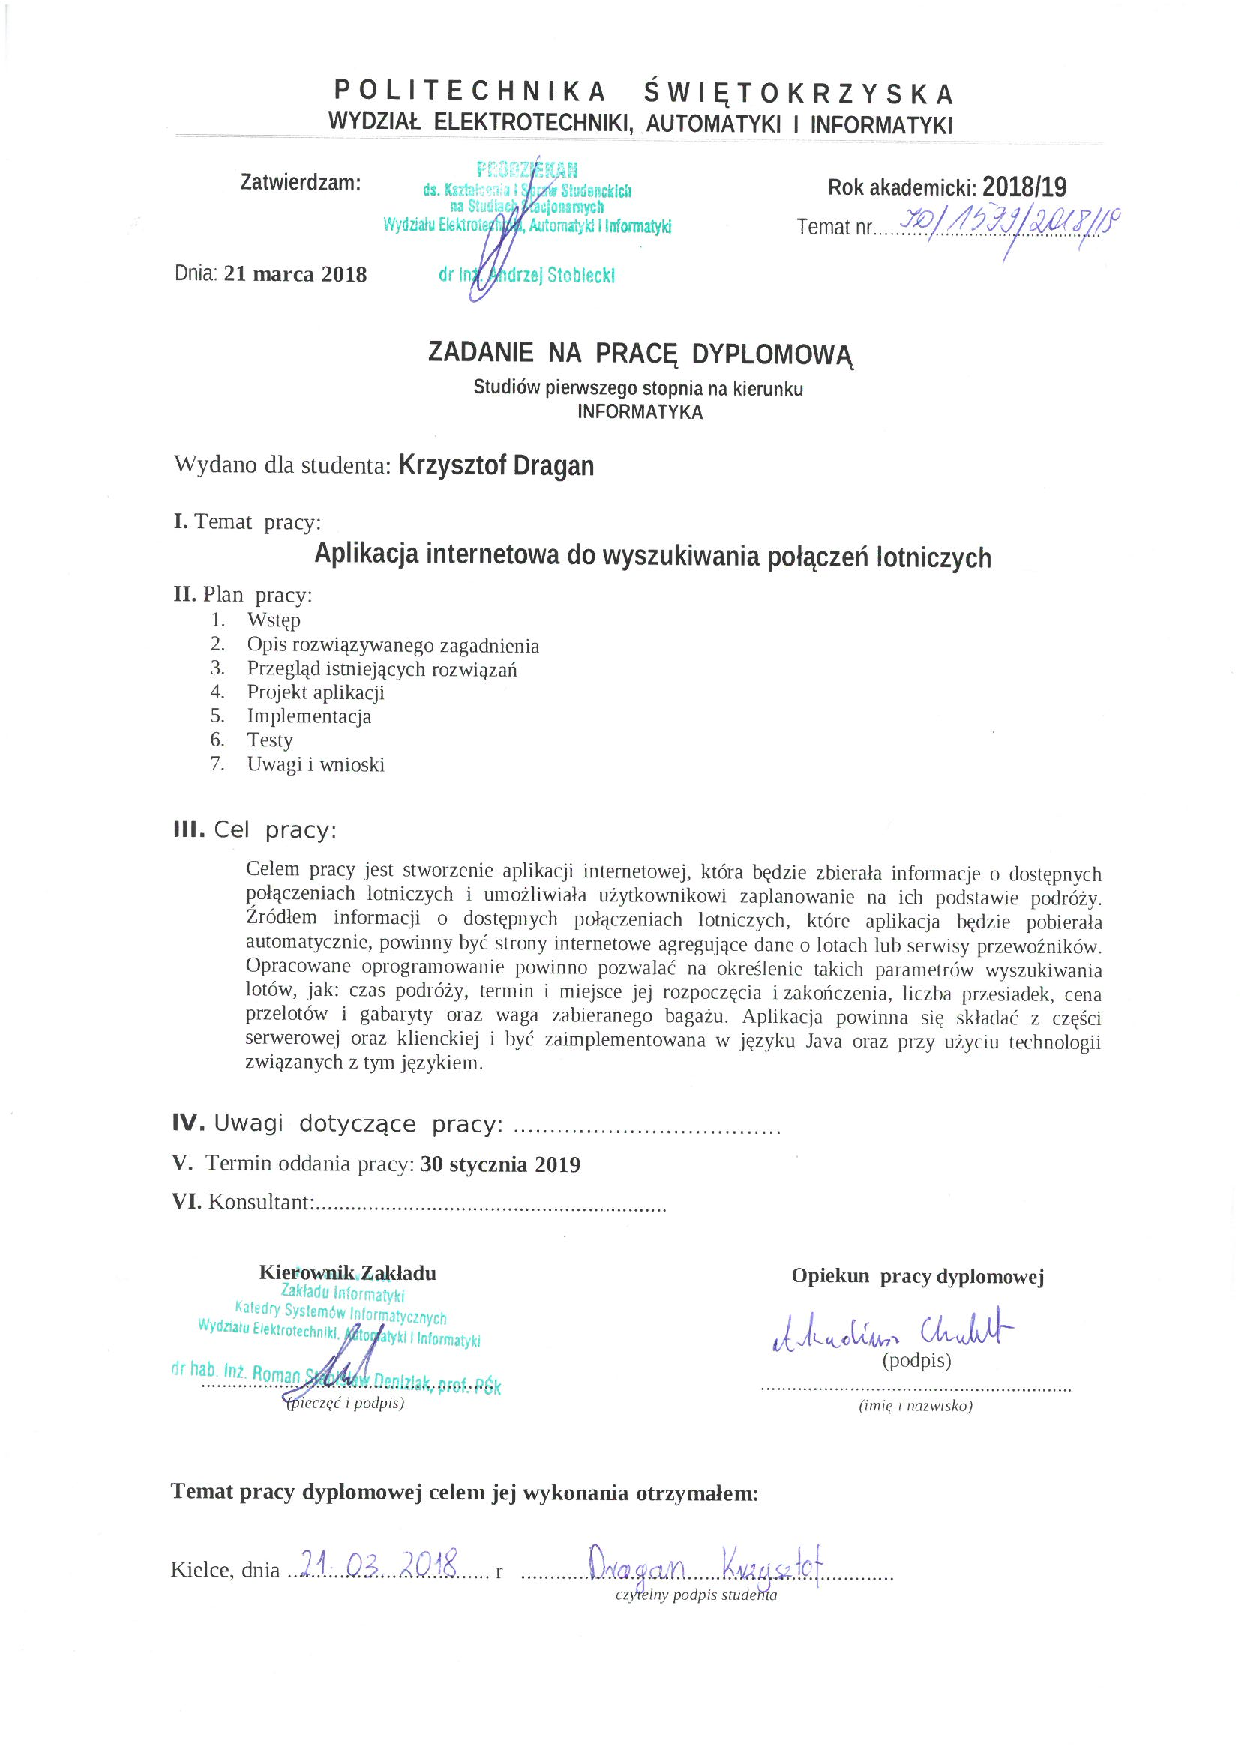
\includepdf[pages=-]{docs/zadanie.pdf}

% --------------------------------------------
% ---------------- Oświadczenie --------------
\afterpage{\blankpage}

\includepdf[pages=-]{docs/oswiadczenie.pdf}  

% --------------------------------------------
% --------------- Streszczenie ---------------
\newpage
\thispagestyle{empty}
\begin{center}
	{\fontsize{14pt}{12pt}\selectfont
		\textbf{Aplikacja internetowa do wyszukiwania połączeń lotniczych}}
\end{center}

\begin{flushleft}
	{\fontsize{14pt}{12pt}\selectfont
		\textbf{Streszczenie}}\\
	\vspace{1cm}
\tab Celem niniejszej pracy było opracowanie aplikacji internetowej która pozwoliłaby na wyszukiwanie połączeń lotniczych korzystając z danych zawartych na stronach internetowych przewoźników bądź z innych centr danych. Aplikacja została podzielona na część kliencką oraz serwerową. Klient został napisany przy użyciu technologii Angular 6, natomiast część serwerowa w technologii Java 10. W pracy znajduje się opis architektury stworzonej aplikacji, modułu wyszukiwania połączeń lotniczych a także zagadnień teoretycznych związanych z projektowaniem interfejsu użytkownika dla przeglądarki internetowej.
\end{flushleft}
\vspace{0.5cm}
Słowa kluczowe: Java, Angular 6, REST, programowanie obiektowe, protokół HTTP, programowanie funkcyjne

\vspace{1.5cm}

\begin{center}
	{\fontsize{14pt}{12pt}\selectfont
		\textbf{A web application to search for flight connections}}
\end{center}

\begin{flushleft}
	{\fontsize{14pt}{12pt}\selectfont
		\textbf{Summary}}\\
	\vspace{1cm}
\tab The purpose of thesis was to build a web application, which will be able to search flight connections using data included on air websites or other data sources. Application was divided into two parts: client and server. Client was implemented using technology of Angular 6, whereas server in Java 10 technology. Description of architecture built application, module of air connections searching and theoretical issues related to building user interface for web application are included in this thesis. 
\end{flushleft}
\vspace{0.5cm}
Keywords: - Java, Angular 6, REST, Object Oriented Programming, HTTP Protocol, Functional Programming
\afterpage{\blankpage}

% ---------------- Spis Treści ---------------
\renewcommand{\contentsname}{Spis treści}
\newpage
\pagenumbering{arabic}
\setcounter{page}{9}
% Ustawia numerację strony od aktualnej na numer 9
\tableofcontents
% ------------------- Wstęp ------------------
\newpage
\chapter*{Wstęp}
\addcontentsline{toc}{chapter}{Wstęp}
Branża lotnicza to jedna z głównych gałęzi dzisiejszego transportu. Za jej początek uznaje się pierwszy pomyślny lot braci Wright 17 grudnia 1903 roku na polach Kitty Hawk. To wydarzenie zapoczątkowało proces tworzenia się przemysłu lotniczego. W dzisiejszych czasach transport lotniczy uznaje się za najszybszy i najbardziej bezpieczny. Wykorzystuje się go między innymi w transporcie osób, towarów lub też w celach militarnych. Warto wspomnieć też o jego roli jako prekursora lotów kosmicznych. Dzięki niemu powstała nieosiągalna wcześniej możliwość podróżowania po całym świecie w możliwe najkrótszym czasie.\\
\indent W niniejszej pracy podjęto się stworzenia aplikacji internetowej umożliwiającej wyszukiwanie realnych połączeń lotniczych. Aplikacja ta składa się z części klienckiej oraz serwerowej. Dla zwiększenia jej wydajności do architektury została dodana relacyjna baza danych oraz mechanizmy cachowania danych.
Jej główną funkcjonalnością jest zbieranie danych o połączeniach lotniczych z zewnętrznych serwisów oraz zasobów internetowych. 
 Pozwala ona na uzyskanie informacji o lotach uwzględniając dane o ich cenie, linii lotniczej go obsługującej, wymiarów i wagi dozwolonego bagażu, czasu podróży czy też liczby przesiadek.\\
\indent
Praca została podzielona na 6 rozdziałów. Rozdział pierwszy przedstawia zagadnienie wyszukiwania połączeń lotniczych wraz z opisem najważniejszych problemów które podjęto rozwiązaniu podczas powstawania aplikacji. Drugi rozdział opisuje obecnie istniejące rozwiązania na rynku. Jest to opis dwóch komercyjnych aplikacji które zyskały duże uznanie swoich użytkowników. Zakończony został podsumowującym porównaniem obu aplikacji. Rozdział trzeci przedstawia projekt aplikacji. Znajdują się w nim schematy z opisem, które przestawiają architekturę powstałej aplikacji. Obrazuje podział funkcjonalności między bazą danych, warstwą logiki biznesowej czy też warstwą prezentacji. Opisane zostały również ścieżki komunikacji pomiędzy tymi warstwami.
Rozdział czwarty przedkłada implementację aplikacji. W rozdziale tym zostaną przedstawione najważniejsze fragmenty oprogramowania tworzące funkcjonalność aplikacji. Można będzie w nim znaleźć informacje o użytych technologiach jak i zewnętrznych bibliotekach którymi się posłużono. Piąty rozdział poświęcony jest testom oprogramowania, które potwierdzają prawidłowe działanie aplikacji. Ostatni rozdział przedstawia uwagi i wnioski odnoszące się do tematu pracy oraz stworzonej aplikacji.

\newpage
\chapter{Opis rozwiązywanego zagadnienia}
Głównym zagadnieniem podjętym w pracy było  pozyskanie realnych danych o połączeniach lotniczych które można by było zaprezentować w kompleksowym interfejsie oraz we względnie optymalnym czasie dla użytkownika powstałej aplikacji.
Zagadnienie to można podzielić na 3 części:
\begin{itemize}[noitemsep,topsep=0pt]
\item Znalezienie źródeł danych o połączeniach lotniczych
\item Parsowanie różnych rodzajów danych
\item Zapewnienie dobrej wydajności podczas wyszukiwania połączeń lotniczych
\end{itemize}
Części te zostaną opisane w podrozdziałach bieżącego rozdziału.

\section{Źródła danych o połączeniach lotniczych}
Największą trudnością podczas pisania pracy było znalezienie odpowiednich zasobów danych które, nie byłyby płatne oraz które zapewniałyby rzetelne i sprawdzone dane lotnicze. Poszukiwania zaczęto od złożenia podań do centr danych o dostęp do ich zasobów. Większość z nich wymagała opłaty za swoje usługi które sięgały nawet 10 000\$. Niektóre z nich oferowały jednak darmowy dostęp do ich zasobów, jednak był to dostęp limitowany. Na potrzeby pracy wybrano serwis FlightLookup jako głównego dostawcę danych. Informacje przez niego dostarczone stanowiły lwią część odpowiedzi serwera. Darmowy dostęp jest limitowany 500 zapytaniami w trakcie miesiąca.
\vspace{1.0cm}
\begin{figure}[!ht]
\centering

\includegraphics[scale=0.50, keepaspectratio]{flightlookup.png}
\caption{Portal serwisu FlightLookup}
\label{fig:flightlookup}
\end{figure}
\newpage
Dodatkowymi źródłami danych były:
\begin{itemize}[noitemsep,topsep=0pt]
\item Skyscanner - serwis udostępniające średnie ceny przelotów w określonym przedziale czasowym oraz informacje dotyczące dozwolonego bagażu
\item Aviation Edge - usługa chmurowa udostępniające dane o liniach lotniczych 
\item ourairports.com - strona internetowa umożliwiające pobranie danych o większości lotnisk na świecie
\end{itemize}

Skyscanner jest komercyjną aplikacją zbierającą wiele rodzajów danych lotniczych. Jej szczegółowa funkcjonalność zostanie opisana w następnym rozdziale. W tej części pracy zostanie opisane użycie zasobów tego produktu. Zasoby Skyscanner'a dostarczyły danych o aktualnych cenach wyszukiwanych lotów oraz danych dotyczących dozwolonego bagażu podczas podróży. Ceny lotów zostały pobrane z serwisu RapidApi korzystającego wewnętrznie z zasobów aplikacji Skyscanner. Znajduje się on pod adresem sieciowym: \url{https://rapidapi.com/skyscanner/api/skyscanner-flight-search}.\\
Użycie jego serwisów wymagało podania miejsca jak i daty wylotu oraz przylotu. Dodatkowym wymaganym parametrem był unikalny kod walutowy który umożliwiał zwrócenie poprawnych wyników. Oprócz cen przelotów Skyscanner posiada też stronę internetową z tabelą opisującą dozwolone wymiary oraz wagę bagażu podczas przelotu. Adres tej strony to: \url{www.skyscanner.net/news/tips/check-in-luggage-size-and-weight-restrictions}\\
Zawartość tej strony jest parsowana przez część serwerową jednak to zagadnienie zostanie opisane szerzej w następnym podrozdziale.\\ \indent
Kolejnym ważnym źródłem danych jest usługa chmurowa Aviation Edge. Serwis ten w przejrzysty sposób udostępnia dane o liniach lotniczych wykorzystując do tego interfejs REST\footnote{Representational state transfer}. Do użycia tej usługi wymagane było podanie unikalnego kodu linii lotniczej w celu jej zidentyfikowania oraz pobrania danych w postaci JSON. Aviation Edge jest bezpłatnym serwisem, do korzystania z jego zasobów wymagane jest tylko założenia konta w celu uzyskania klucza identyfikującego użytkownika. \\ \indent
Ostatnim źródłem danych jest strona internetowa ourairport.com znajdująca się pod adresem internetowm: \url{http://ourairports.com/}. Jej zasobem który został wykorzystany jako źródło danych jest plik csv zawierający ponad 50000 rekordów lotnisk. Zawiera dane z szerokiego przekroju typów lotnisk począwszy od małych lotnisk dla awionetek aż po największe lotniska świata takie jak London Heathrow Airport. Dane te zabrane są w całości w postaci pliku CSV który jest pobierany przez część serwerową. Poddawane są procesowi filtracji w celu wyeliminowania lotnisk obsługujących poniżej 4 tysięcy pasażerów rocznie.
\newpage
\section{Parsowanie różnych rodzajów danych}

Dane dostarczone przez zewnętrzne serwisy prezentowały swoją treść w różnych formatach. Aby zebrać pełną odpowiedź serwera należało w pierwszym kroku sparsować pojedyncze elementy a następnie zbudować z nich obiekt języka Java.
\subsection{Język znaczników XML}
XML\footnote{eXtensible Markup Language} to standard oznaczeń popierany przez organizację W3C. Definiuje on ogólną składnię, stosowaną przy oznaczaniu danych za pomocą prostych znaczników.\cite{xml} Ponadto oferuje standardowy format dokumentów komputerowych. Format ten można dostosowywać do dziedzin tak odmiennych jak witryny WWW, wymiana danych elektronicznych, grafika wektorowa, serializacja obiektów czy systemy poczty głosowej. Dane w dokumentach XML są zapisywane w postaci ciągów tekstowych, zawartych w oznaczeniu tekstowym opisującym te dane. Poszczególne jednostki danych i oznaczenia nazywane są elementami. Specyfikacja XML określa, jakie wymogi składniowe musi spełniać takie oznaczenie: w jaki sposób elementy są rozgraniczane przez znaczniki, jak wygląda znacznik, jakie nazwy elementów są akceptowanie, gdzie trzeba umieszczać atrybuty i tak dalej. Oznaczenia dokumentu XML są bardzo podobne do oznaczeń dokumentów HTML, choć występują między nimi pewne różnice.

\begin{lstlisting}[language=XML, caption=Fragment danych w formacie XML]
    <FlightDetails TotalFlightTime="PT3H35M"
                   TotalMiles="931"
                   TotalTripTime="PT4H25M"
                   FLSDepartureDateTime="2018-11-15T06:40:00"
                   FLSDepartureTimeOffset="+0100"
                   FLSDepartureCode="WAW"
                   FLSDepartureName="Warsaw"
                   FLSArrivalDateTime="2018-11-15T10:05:00"
                   FLSArrivalTimeOffset="+0000"
                   FLSArrivalCode="LHR"
                   FLSArrivalName="London Heathrow"
                   FLSFlightType="Connect"
                   FLSFlightLegs="2"
                   FLSFlightDays="...4..."
                   FLSDayIndicator=""
    >
\end{lstlisting}
\newpage
XML jest wyłącznie językiem znaczników, nie jest on ani językiem programowania, protokołem transportu sieciowego czy też bazą danych. XML oferuje możliwość formatowania danych, zapewnia to ich prawdziwą wieloplatformowość i odporność na upływ czasu. Dotychczas dokument zapisany za pomocą jakiegoś oprogramowania na jednej platformie nie dawał się odczytywać na innej platformie ani na zbliżonej platformie za pomocą innego rodzaju oprogramowania. 

Wyszukiwanie informacji o połączeniach lotniczych zaczynało się od odebrania danych z serwisu FlightLookup w postaci XML. Jest to najważniejsza operacja podczas procesu wyszukiwania połączeń lotniczych. Dane zebrane w tej części są parametrami wyszukiwania podczas korzystania ze źródeł danych wykorzystanych w późniejszym etapie tego procesu. Przykład odebranej treści znajduje się na listingu 1.2.1 załączonym na poprzedniej stronie.

Operacja parsowania obiektów XML na obiekty języka Java zostanie szerzej opisana w rozdziale o implementacji. Załączony listing 1.2.1 przedstawia jeden z elementów danych XML o nazwie \textit{FlightDetails}. Zawiera on przykładowe pola takie jak: \textit{TotalMiles} czy \textit{FLSFlightDays}. Elementy te zostały odwzorowane w postaci klas języka Java o takich samych nazwach jak nazwa elementu. Powstała klasa posiada też takie same pola jak obiekt w XML.
\subsection{Notacja JSON}
Notacja JSON\footnote{JavaScript Object Notation} jest modernistycznym sposobem prezentacji danych. Wywodzi się ona z języka JavaScript gdzie została głównym formatem prezentacji obiektów tej technologii. Notacja Json jest zbudowana na dwóch strukturach\cite{json}:
\begin{itemize}[noitemsep,topsep=0pt]
\item Kolekcji par nazwa/wartość, w zależności od języka programowania zrealizowana jako obiekt, rekord, struktura, słownik bądź kolekcja
\item Posortowana lista wartości. W większości języków zrealizowana jako tablica, wektor, lista lub sekwencja
\end{itemize}
Są to uniwersalne struktury danych. Wirtualnie wszystkie nowoczesne języki programowania wspierają je w specyficznej dla siebie formie. Notacja JSON jest to format danych, który jest wymienny z językami programowania. Ta właściwość czyni ją najpopularniejszym formatem wymiany danych między aplikacjami oraz mikroserwisami. W stworzonej aplikacji dane w tym formacie dotyczyły liniach lotniczych oraz cen przelotów. W pierwszym przypadku obiekt JSON można było w prosty sposób skonwertować na obiekt języka Java. Przykładową strukturę zaprezentowano na listingu 1.2.3\\
Kod odpowiedzialny za konwersję tego obiektu zostanie przedstawiony w rozdziale piątym.
\newpage
\begin{lstlisting}[language=JSON, caption= Przykładowy obiekt w notacji JSON]
   [
    {
        "airlineId": "1",
        "nameAirline": "American Airlines",
        "codeIataAirline": "AA",
        "iataPrefixAccounting": "1",
        "codeIcaoAirline": "AAL",
        "callsign": "AMERICAN",
        "type": "scheduled",
        "statusAirline": "active",
        "founding": "1934",
        "codeHub": "DFW",
        "nameCountry": "United States",
        "codeIso2Country": "US"
    }
]
\end{lstlisting}
\subsection{Język HTML}
HTML\footnote{Hypertext Markup Language} jest standardowym językiem znaczników dla tworzenia stron internetowych\cite{html}. Dokumenty HTML są podstawową treścią jaką generują przeglądarki internetowe. W pracy dyplomowej źródłem danych o wymiarach i wadze dozwolonych bagaży była strona internetowa aplikacji Skyscanner. Poniżej przedstawiono fragment danych zapisanych w formacie HTML które posłużyły do celów pracy.
\begin{lstlisting}[language=HTML5, caption= Fragment dokumentu HTML]
<table class="tftable" style="height: 3990px" border="1" width="578">
<tbody>
<td><a href="https://www.skyscanner.net/news/tips/aer-lingus-baggage-allowance-explained/">Aer Lingus</a></td>
<td>No free allowance</td>
<td>No size restriction
<p>&nbsp;</p>
<p><strong>32kg</strong> per bag, or<br>40kg across 2 bags</p>
</td>
</tr>
<tr>
\end{lstlisting}

\newpage
\section{Wydajność wyszukiwania}
Wyszukiwanie tak złożonych danych jak informacje o połączeniach lotniczych, a następnie parsowanie ich niesie za sobą pewne konsekwencje. Są to konsekwencje czasowe, użytkownik powinien otrzymać interesującą go treść w czasie jak najkrótszym. W celu optymalizacji wydajności aplikacji wprowadzono mechanizmy skracające czas odpowiedzi części serwerowej.
Dla zbierania danych dotyczących lotnisk oraz bagażów wprowadzono rozwiązania polegające na pobieraniu pełnych zasobów tych danów do bazy danych lub do pliku tekstowego znajdującego się na serwerze. Pozwoliło to na pominięcie opóźnienia sieciowego związanego z potencjalną koniecznością pobierania tych danych ze stron lub zewnętrznych baz danych.\\ \indent
Kolejnym rozwiązaniem było wprowadzenie funkcyjnego stylu programowania w kluczowych elementach części serwerowej które odpowiadały za wyszukiwanie połączeń lotniczych.  Programowanie funkcyjne wprowadzone w Javie 8 pozwala skrócić operacje po stronie wirtualnej maszyny Javy,a więc też zaoszczędzić cenne milisekundy w trakcie wyszukiwania lotów.
Implementacje tych rozwiązań znajdują się w rodziale czwartym.\\ \indent
Ostatnim mechanizmem był rozwiązanie cachowania danych. Caching jest mechanizmem przyspieszającym działanie aplikacji oraz zwiększającym ogólną wydajność. Część danych która jest gromadzona w aplikacji o długich czasach dostępu i niższej przepustowości jest dodatkowo przechowywana w pamięci RAM o lepszych parametrach\cite{ehcache}. Pamięć RAM inaczej nazywana jest też pamięcią podręczną. Jest podstawą wszystkich nowoczesnych systemów informatycznych. Odczytywanie danych z tej pamięci jest najszybsze porównując go na przykład z odczytywaniem z dokumentów XML, JSON, bazy danych czy też zasobów sieciowych. Jego przeznaczeniem jest skracanie czasu odpowiedzi dla określonych zapytań do części serwerowej,które są zwielokrotnione i wywoływane przez wielu użytkowników. Wykonując operacje wyszukiwania lotów, moduł wyszukiwania sprawdza czy w cache'u znajdują się poszukiwanie operacje. Jeśli tak, zwraca je użytkownikowi. W przeciwnym wypadku  wyszukuje loty standardowym sposobem a wynik zapisuje do cache'u. Dla danych o liniach lotniczych, bagażach oraz dla całego obiektu lotu w części serwerowej stworzono 3 kontenery cache'u. Czas przetrzymywanie danych w tych kontenerach wynosi odpowiednio: 7 dni, 3 dni oraz 3 godziny. Przy wyborze informacji które powinny znaleźć się w pamięci podręcznej sugerowano się temperaturą danych. Trzy wcześniej wymienione zasoby oceniono z największym prawdopodobieństem na ich użycie przez użytkowników aplikacji.
Jednostki te wybrano uwzględniając wrażliwość tych danych na ciągłe zmiany w systemach lotniczych. Implementacja tych mechanizmów wraz z kodem źródłowym znajduje się w rozdziale czwartym.
\newpage
\chapter{Przegląd istniejących rozwiązań}
Analiza istniejących rozwiązań, aplikacji wyszukujących połączenia lotnicze pozwoliła nadać pracy bardziej precyzyjne wymagania oraz zaprojektować jej ogólny przebieg. W internecie można znaleźć wiele aplikacji o podobnych lub takich samych funkcjonalnościach jak opracowana praca. W tym rozdziale zostaną opisane najbardziej znane wyszukiwarki lotów dostępnych na rynku. 
\section{Wyszukiwarka lotów Skyscanner}
Pierwszym przykładem została aplikacja internetowa Skyscanner. Jest to wyszukiwarka lotów, która umożliwia użytkownikom szukanie lotów według ceny i lokalizacji. Oprócz funkcji wyszukiwania lotów, Skyscanner oferuje opcje wyszukiwania hotelów blisko lotnisk oraz wypożyczenia auta w pobliżu lotniska docelowego. Aplikacja ta została stworzona oraz wdrożona w 2002 roku. Od tego czasu firma Ctrip która jest właścicielem tego produktu zatrudnia ponad 200 pracowników. Warto wspomnieć o jej innej usłudze która udostępnia dane o połączeniach lotniczym zewnętrznym firmom i deweloperom. Jej dane były brane pod uwagę w czasie szukania źródeł danych lecz Skyscanner wymaga dużych opłat za swoje usługi, w warunkach akademickich niemożliwe było z ich skorzystanie.
Aplikacja ta jest dostępna w ponad 30 językach oraz używana przez 60 milionów użytkowników miesięcznie. Aplikacja wiele razy nagradzana była za swoją funkcjonalność i użyteczność użytkownikom. Skyscanner znajduje się pod adresem sieciowym: 
\url{https://www.skyscanner.net/}.\\ \indent
Opisywana aplikacja ma dla swoich użytkowników szereg przydatnych funkcjonalności. Korzystające z jej osoby mogą korzystać z kompleksowego modułu wyszukiwania połączeń lotniczych. W panelu wyboru parametrów lotów można wybrać lotnisko wylotu, lotnisko docelowe jak i daty wylotu. Skyscanner oferuje 3 sposoby wyszukiwania lotów: lot powrotny, lot w jedną stronę oraz podróż wieloetapowa. Dodatkowo użytkownik jest w stanie sprecyzować liczbę osób podczas podróży jak i klasę biletu lotniczego. Ciekawą funkcjonalnością jest możliwość dodania pobliskich lotnisk do tych wybranych przez użytkownika. Znajduje ona zastosowanie, gdy na przykład aplikacja nie może znaleźć lotów z wybranego lotniska. Następuje wtedy wyszukiwanie lotów z pobliskich lotnisk o zadanym promieniu odległości.
Oprócz bogatego interfejsu do wyboru parametrów lotów Skyscanner oferuje bardzo dobrą wydajność podczas wyszukiwania. Loty bezpośrednie wyszukiwane są natychmiastowo. Na loty z zaznaczoną opcja możliwych przesiadek trzeba poczekać kilka sekund. Interfejs aplikacji Skyscanner zostanie zaprezentowany na następnej stronie.
\newpage
\begin{figure}[!ht]
\centering
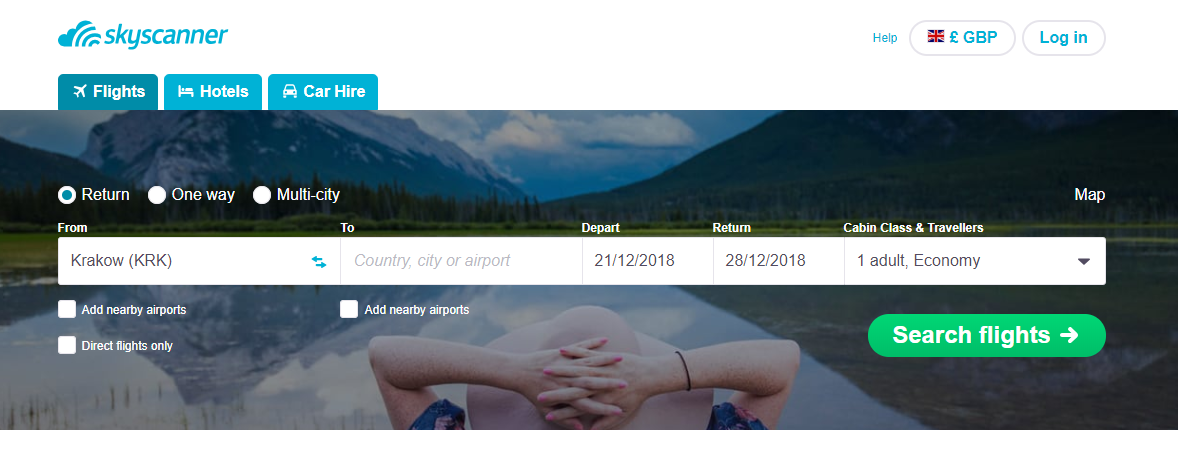
\includegraphics[scale=0.50, keepaspectratio]{skyscanner_main.png}
\caption{Panel wyszukiwania lotów aplikacji Skyscanner}
\label{fig:skyscanner_main}
\end{figure}
Po wybraniu odpowiednich parametrów należy nacisnąć zielony przycisk po prawej aby rozpocząć 
proces wyszukiwania lotów. Jego przykładowe wyniki zaprezentowano na rysunku 2.1.2, można na nim zauważyć wyszukane loty z dokładnymi informacjami o linii lotniczej obsługującej lot, miejsca wylotu oraz przylotu, czasie podróży jak i liczbie przesiadek. Z lewej strony dostępny jest panel dzięki któremu można dokonać różnego rodzaju filtracji na otrzymanych wynikach.
\begin{figure}[!ht]
\centering
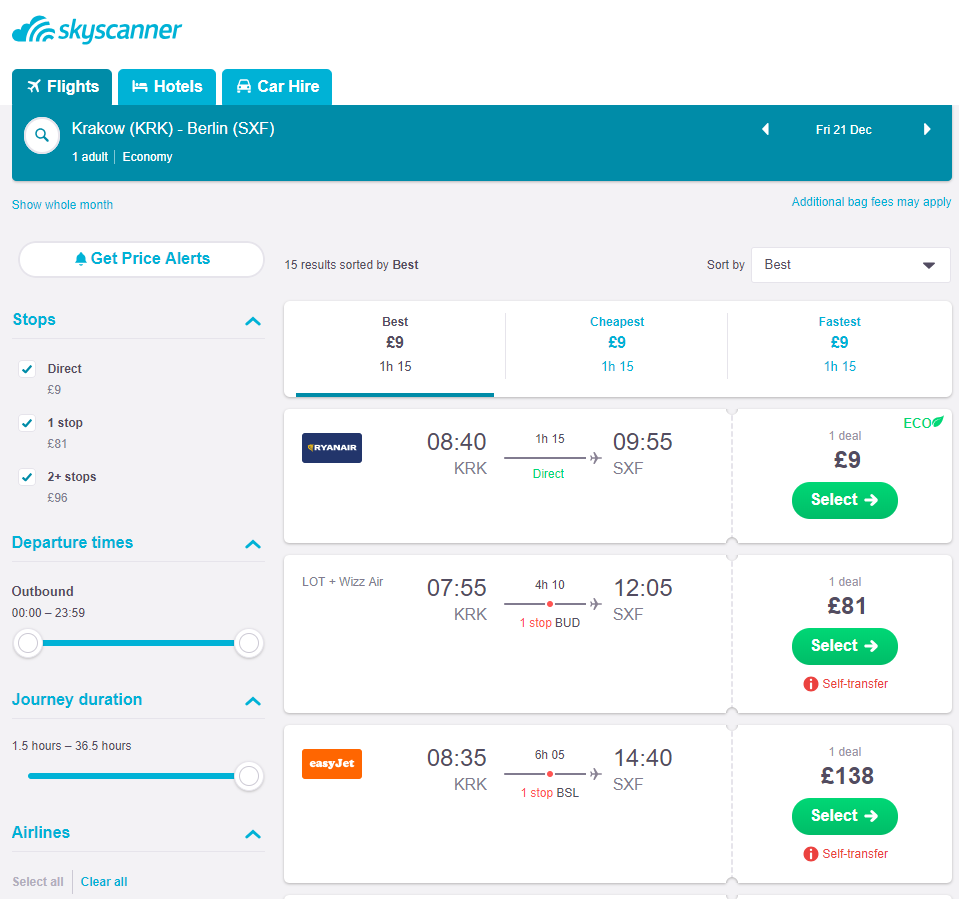
\includegraphics[scale=0.45, keepaspectratio]{skyscanner_result.png}
\caption{Wyniki wyszukiwania lotów aplikacji Skyscanner}
\label{fig:skyscanner_result}
\end{figure}


\newpage
Warto zwrócić uwagę na panel podróży wieloetapowej, który jest dostępny po kliknięciu  odpowiedniego przycisku powyżej pola do wyboru lotniska wylotowego. Można w nim wybrać do siedmiu osobnych połączeń lotniczych i na ich podstawie zaplanować swoją podróż. Każde z tych połączeń jest domyślnie połączeniem w jedną stronę. 
\begin{figure}[!ht]
\centering
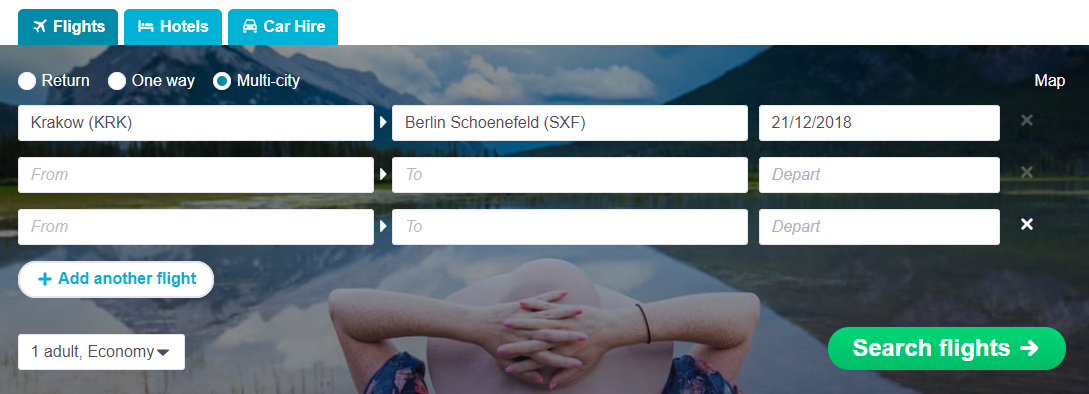
\includegraphics[scale=0.50, keepaspectratio]{skyscanner_multi.png}
\caption{Komponent podróży wieloetapowej}
\label{fig:skyscanner_multi}
\end{figure}

\section{Wyszukiwarka lotów Google Flights}
Kolejnym przedstawianym rozwiązaniem jest aplikacja internetowa Google Flights firmy Google. Jest to jeden z głównych internetowych produktów giganta z Kalifornii.W pełni integruje się z innymi usługami tej firmy co czyni go bardzo praktycznym systemem. Google Flights zostało wdrożone 13 października 2011 roku. Ma zbliżone funkcjonalności do wcześniej opisywanego konkurenta Skyscanner. Oferuje jednak pewne innowacje. Pozwala użytkownikowi na wyszukiwanie lotów określając okres czasowy go interesujący oraz budżet na jaki pozwala jego portfel. Największą zaletą tej aplikacji jest jej szybkość. Dzięki spokrewnieniu z silnikiem Google Search szybkość wyszukiwania połączeń lotniczych jest bezkonkurencyjna na rynku wyszukiwarek lotów. Szybkość ta została uzyskana przez użycie wyspecjalizowanych algorytmów szukających firmy Google oraz specjalnemu indeksowaniu danych.
Oprócz samej funkcjonalności aplikacja prezentuje czytelny i responsywny interfejs, który zyskał aprobatę ze strony użytkowników.


\begin{figure}[!ht]
\centering
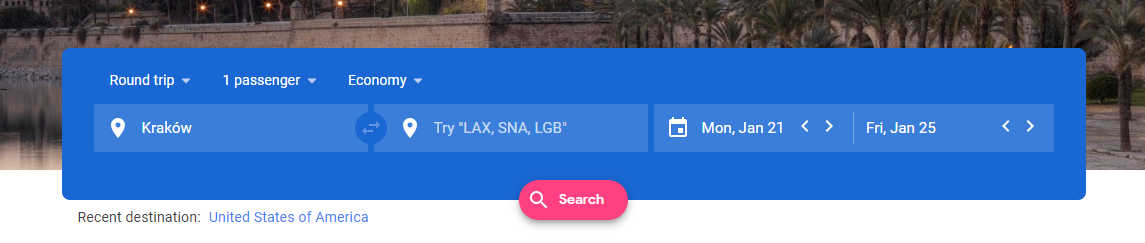
\includegraphics[scale=0.50, keepaspectratio]{google_flights_search_panel.png}
\caption{Panel wyszukiwania lotów aplikacji Google Flights}
\label{fig:google_flights_search_panel}
\end{figure}
Na rysunku 2.2.1 przedstawiono panel wyszukiwania lotów oferowany przez opisywaną aplikację. Dostępny jest też komponent podróży wieloetapowej który znalazł się też w poprzednio opisywanej aplikacji oraz w części praktycznej tej pracy.

\begin{figure}[!ht]
\centering
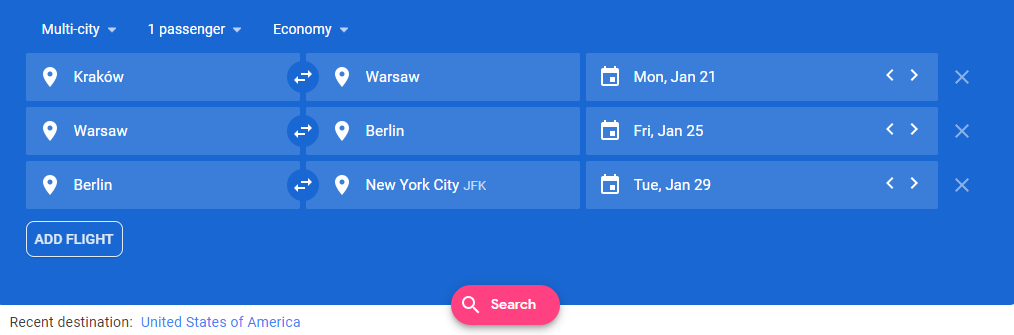
\includegraphics[scale=0.60, keepaspectratio]{google_flights_multi.png}
\caption{Komponent podróży wieloetapowej aplikacji Google Flights}
\label{fig:google_flights_multi}
\end{figure}
Wszystkie produkty firmy Google, które można obejrzeć w przeglądarce internetowej charakteryzują się specyficznym stylem interfejsu. Jest to platforma Material Design, która wyznacza specyfikację pojedynczych elementów aplikacji Google'a. Rysunek 2.2.3 przedstawia przykładowe wyniki wyszukiwania lotów. Wyszukane loty znajdują się w rozwijanej liście. Po kliknięciu w wybrany element listy rozwija się panel z dokładniejszymi informacjami o locie. Każdy element zaprezentowany na poniższym rysunku jest zgodny z wcześniej wspomnianą platformą Material Design. Widać na przykład zaokrąglenia przycisków charakterystyczne dla produktów marki Google.
 
\begin{figure}[!ht]
\centering
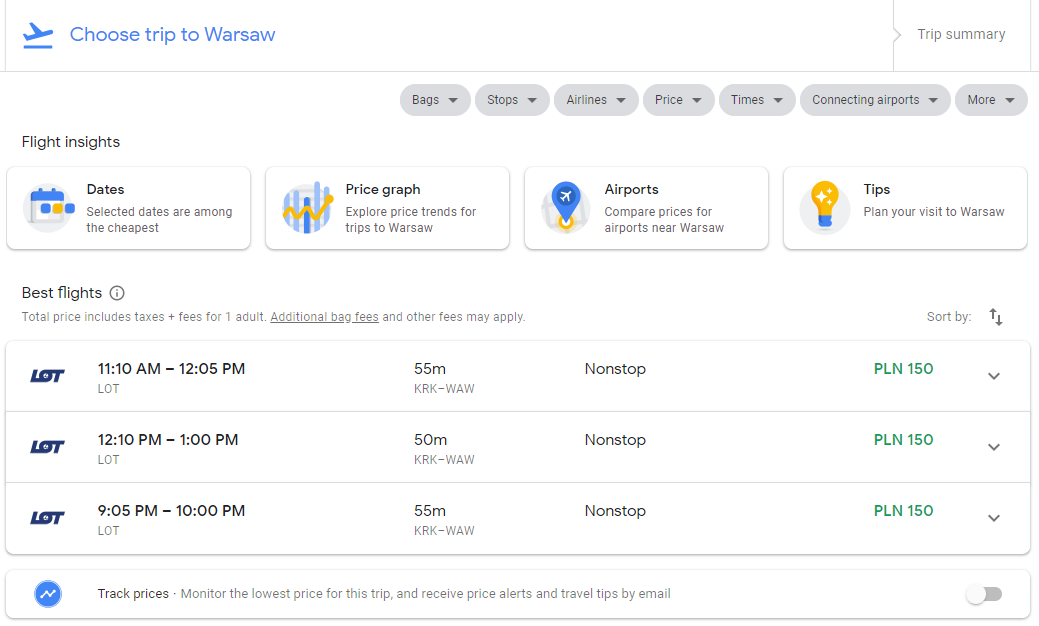
\includegraphics[scale=0.50, keepaspectratio]{google_flights_result.png}
\caption{Komponent podróży wieloetapowej aplikacji Google Flights}
\label{fig:google_flights_multi}
\end{figure}

\newpage
\section{Porównanie aplikacji}
Obie opisane aplikacje są rozwiązaniami komercyjnymi, stworzonymi przez wieloosobowe zespoły programistów. Są systemami sprawnie działającymi, z czytelnym oraz zrozumiałym interfejsem graficznym. Swoją funkcjonalnością są do siebie identyczne, posiadają tą samą ofertę dla użytkownika jednak różnią się jakością jej wykonania. \\ \indent
Zaletami aplikacji Skyscanner jest z pewnością rzetelność jej danych. Jest to potwierdzone ze strony linii lotniczych, które wielokrotnie nagradzały tą aplikację. Warto też wspomnieć o jej systemie wyszukiwania lotów. Ilość wyszukanych lotów z przesiadkami często przekracza 100 wystąpień. Świadczy to o zaawansowanym silniku wyszukującym i analizującym różne przypadki połączeń. Za wady można uznać dosyć prosty i nieresponsywny interfejs użytkownika. Nie reprezentuje on poziomu nowoczesnych aplikacji. \\ \indent
Druga wyszukiwarka jest bardzo dopracowanym produktem światowego giganta. Jak wcześniej już wspomniano jego szybkość wyszukiwania danych jest bezkonkurencyjna. Aplikacja Skyscanner znacznie ustępuje jej na tym polu. Google Flights jest sprzężona z systemami sprzedażowymi większości przewoźników lotniczych. Daje to możliwość kupna biletu bezpośrednio z jej poziomu bez konieczności przechodzenia na zewnętrzną stronę linii lotniczej. Jej dużą zaletą z pewnością jest dopracowany interfejs zgodny ze standardami reprezentowanymi w rodzimych produktach. Gwarantuje on pełną responsywność oraz czytelność prezentowanych danych. \\ \indent
Wyszukiwarka Google Flights prezentuje się lepiej od aplikacji Skyscanner jednak różnica je dzieląca nie jest duża. W opracowywanej aplikacji starano się w rzetelny sposób zrealizować podstawowe funkcjonalności obu opisywanych wcześniej aplikacji. Komercyjne aplikacje mają dużą przewagę biorąc pod uwagę szybkość wyszukiwania. W powstałej aplikacji czas odpowiedzi na żądania użytkownika jest zauważalnie większy. W warunkach akademickich trudno było o uzyskanie konkurencyjnych rezultatów.
\newpage

\chapter{Projekt aplikacji}
Następnym krokiem po analizie zagadnienia oraz zaznajomieniem się z przykładami istniejących rozwiązań było opracowanie projektu aplikacji. Zadanie to jest mocno związane z dziedziną architektury oprogramowania. Dobrze zaprojektowany system pozwala na uniknięcie wielu kosztownych problemów w przyszłości. Projektowanie aplikacji wymusza na osobie to wykonującej dostatecznie wczesne rozważenia najważniejszych aspektów projektowania w odniesieniu do całego tworzonego systemu.\cite{architektura}Wynikiem zrealizowania zadań analitycznych są wymagania postawione tworzonemu systemowi. Wynikiem tych działań mogą być takie elementy jak model dziedziny, model wymagań czy model organizacyjny. Na podstawie projektu aplikacji ukierunkowuje się zadania implementacyjne, łącznie z projektowaniem detalicznym, tworzeniem kodu, scalaniem oraz testowaniem.


\section{Ogólna architektura aplikacji}
Projektowanie aplikacji wymagało stworzenia czytelnego schematu obrazującego poszczególne części systemu oraz sposoby komunikacji między nimi.
Aplikację można podzielić na 3 logiczne części: 
\begin{itemize}[noitemsep,topsep=0pt]
\item Część serwerowa
\item Część kliencka
\item Baza danych 
\end{itemize}
Każda część posiada unikalną dla siebie funkcjonalność. 
Ze względu na rozmiar pracy włożony w każde z nich, w tym rozdziale zostaną one krótko opisane.
Część serwerowa w całym systemie jest odpowiedzialna za dostarczenie danych do interfejsu użytkownika inaczej nazywanego częścią kliencką. Znajduje się w nim złożony moduł wyszukiwania połączeń lotniczych. Moduł ten sam w sobie posiada złożoną architekturę i  zostanie mu poświęcony dedykowany podrozdział.
Część kliencka to internetowy interfejs użytkownika. Osadzony jest on w przeglądarce internetowej. W aplikacji nie zdecydowano się na podział względem ról użytkownika. Wynika to ze specyfiki projektowanej aplikacji. Każdy użytkownik ją odwiedzający posiada takie same uprawnienia do jej zasobów.
Oprócz dwóch wspomnianych wcześniej modułów w skład architektury aplikacji wchodzi relacyjna baza danych która jest nośnikiem danych dla tabeli lotnisk.
Kluczowym zagadnieniem jest komunikacja między powyższymi komponentami. W stworzonej aplikacji istnieje kilka rodzajów transportu danych między modułami. Każdy z nich zostanie szczegółowo opisany w dalszej części tego rozdziału.


\begin{figure}[!ht]
\centering
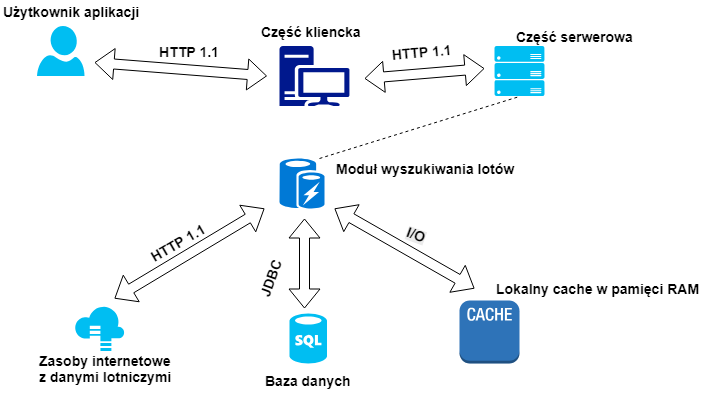
\includegraphics[scale=0.60, keepaspectratio]{architecure_diagram.png}
\caption{Schemat architektury stworzonej aplikacji}
\label{fig:architecure_diagram}
\end{figure}

\newpage
Na rysunku 3.1.1 zamieszczony został schemat architektury stworzonego systemu. Przedstawia on rozdział strukturalny aplikacji oraz drogę jaką musi odbyć żądanie użytkownika w celu uzyskania pożądanej odpowiedzi. Użytkownik po wypełnieniu odpowiednich formularzy w części klienckiej rozpoczyna proces wyszukiwania połączeń lotniczych. Oprogramowanie klienta po pobraniu od użytkownika niezbędnych parametrów takich jak miejsce wylotu, czy rodzaj lotu zwraca się do części serwerowej o wyszukanie lotów zgodnych z podanymi parametrami. Komunikacja między tymi modułami odbywa się protokołem HTTP. Po wywołaniu, część serwerowa zwraca się do modułu wyszukiwania lotów. Moduł ten sprawdza wszystkie źródła danych zamieszczone na schemacie 3.1.1 . Zebrane dane są odpowiednio parsowane i przekazywane modułowi wyszukiwania który z kolei zwraca je kontrolerowi wywołanemu przez użytkownika. Kontroler następnie przekazuje dane do części klienckiej która wyświetla je w  graficznym interfejsie użytkownika. 
\section{Diagram UML}
Kluczowym elementem podczas tworzenia oprogramowania jest komunikacja. Przełożenie złożonej logiki biznesowej na język informatyczny to zadanie trudne oraz wymagające zrozumienia wymagań potencjalnego odbiorcy tworzonej dokumentacji technicznej. Ważny jest więc czytelny sposób opisu oprogramowania, który byłby w stanie zrozumiale przedstawić swoja treść wszystkim osobom się z nim zaznajamiającym. Podstawowym narzędziem w tej dziedzinie stał się język UML\footnote{Unified Modelling Language}.\cite{uml} \\


\begin{figure}[!ht]
\centering
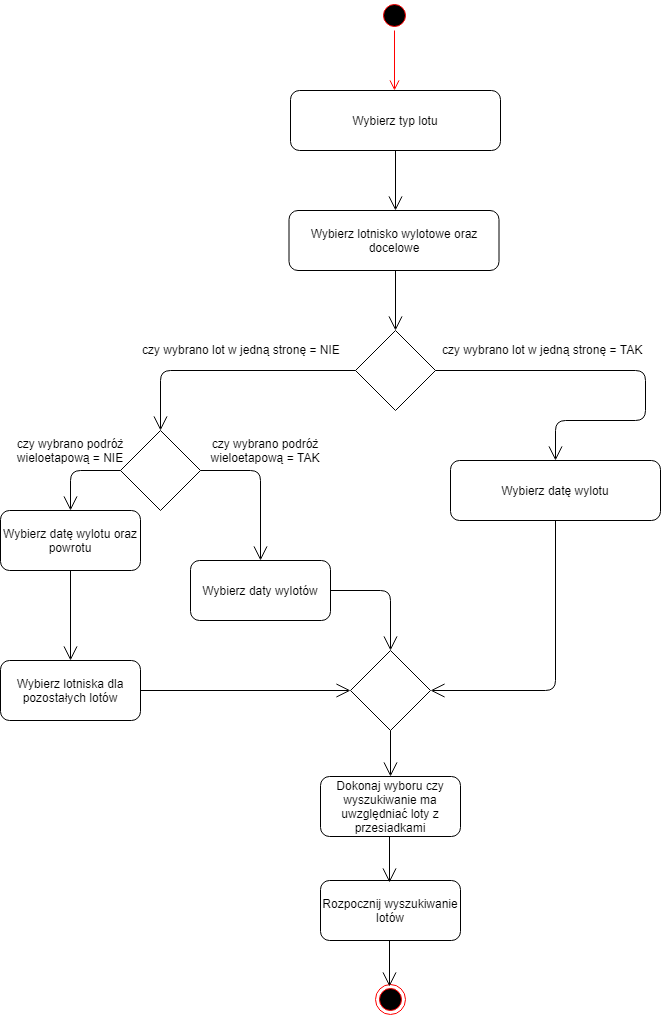
\includegraphics[scale=0.56, keepaspectratio]{activity_diagram.png}
\caption{Diagram aktywności}
\label{fig:architecure_diagram}
\end{figure}
Dla opracowanej aplikacji przygotowano diagram aktywności widoczny na rysunku 3.2.1 Obrazuje on przebieg wydarzeń które wykonywane są przez użytkownika po wczytaniu przez niego strony startowej. Jego najważniejszą funkcją jest ukazanie sekwencji kroków wykonywanych w części klienckiej.
\newpage
\section{Baza danych}
Baza danych nie była sprecyzowana w wymaganiach pracy dyplomowej. Została ona użyta opcjonalnie jako miejsce dające szybki dostęp do danych o lotniskach. Użyto darmowego rozwiązania bazodanowego MySQL. MySQL to system zarządzania bazami danych rozwijany w przeszłości przez firmę MySQL AB, a obecnie przez korporację Oracle. Stanowi szybko działające oprogramowanie i obecnie jest jednym z popularniejszych serwerów baz danych dostępny na licencji GPL\footnote{General Public License} jak i w wersjach komercyjnych \cite{mysql}.

\begin{figure}[!ht]
\centering
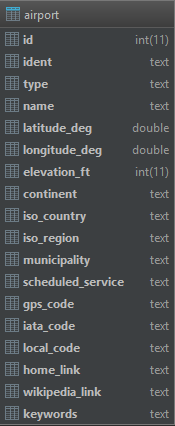
\includegraphics[scale=0.80, keepaspectratio]{database.png}
\caption{Tabela danych lotnisk}
\label{fig:database}
\end{figure}
Jedyna tabela znajdująca się w bazie danych to tabela lotnisk z parametrami wskazanymi powyżej.

\section{Część kliencka}
Aplikacja kliencka została zaimplementowana w technologii Angular 6, otwartym framework'u i platformie do tworzenia SPA\footnote{Single Page Application}. Angular został w całości napisany w języku TypeScript, opiekę nad jego rozwojem sprawuje firma Google. Platforma ta umożliwia tworzenie stron internetowych których treść jest dynamicznie zmieniana bez przeładowywania strony. Przynosi to ogromne korzyści w wydajności aplikacji. Całość kodu napisanego w tym framework'u jest kompilowana do języka JavaScript a następnie renderowana w przeglądarce internetowej. W skład stworzonej aplikacji klienckiej wchodzą dodatkowo dodane zewnętrzne biblioteki.\\ Są to: 
\begin{itemize}[noitemsep,topsep=0pt]
\item Material Design - pakiet oprogramowania od firmy Google do edytowania wyglądu strony
\item MDBootstrap - zestaw narzędzi z gotowymi komponentami do tworzenia stron internetowych
\item NgxSpinner - zewnętrzna biblioteka dodająca komponenty ładowania efektów wizualnych
\item Bootstrap - pakiet oprogramowania do tworzenia responsywnego interfejsu
\end{itemize}
Implementacja częśći klienckiej jak i jej logiczny podział strukturalny znajdzie się w następnym rodziale.

\section{Część serwerowa}
Do opracowania aplikacji serwerowej posłużono się językiem programowania Java w wersji 10 oraz pakietami oprogramowania Spring i Hibernate. Java jest w pełni obiektowym językiem programowania z ponad 20 letnią historią. Pierwotnie stworzona i rozwijana przez Jamesa Goslinga została przejęta przez korporację Oracle. Głównym założeniem tego języka jest sentencja \textit{"Napisz raz, uruchom wszędzie"}. Te słowa przemawiają za specjalnym mechanizmem kompilowania i uruchamiania kodu przez Javę. Proces zaczyna się od skompilowania plików o rozszerzeniu java do bytecode'u czyli specjalnej sekwencji bajtów rozumianej przez JVM\footnote{Java Virtual Machine}. Następnym krokiem jest uruchomienie bytecode'u przez virtualną maszynę Javy nazywaną JVM.\cite{jvm} \\ \indent
Powstałe oprogramowanie serwerowe jest w dużej mierze oparte na zewnętrznych bibliotekach platformy Spring Framework w wersji 5. Spring jest otwartym źródłowo frameworkiem bazującym na wirtualnej maszynie Javy. Jego składowymi jest zbiór bibliotek, których głównym celem jest rozwiązanie popularnych problemów programistycznych. Został stworzony w roku 2002 jako kandydat do zastąpienia oprogramowania spod znaku JavyEE\footnote{Java Enterprise Edition}. W dzisiejszych czasach Spring jest rozwijany przez setki programistów z całego świata co czyni go stale nowoczesną technologią. W części serwerowej Sping Framework odpowiada za komunikację z bazą danych, udostępnienie danych o połączeniach lotniczych aplikacji klienckiej oraz za zabezpieczenia całego systemu. \\ \indent
W części serwerowej w celu przyspieszenia prac programistycznych użyto szeregu zewnętrznego oprogramowania. Należą do nich biblioteki:
\begin{itemize}[noitemsep,topsep=0pt]
\item okhttp - klient protokołu HTTP do pobierania zasobów internetowych
\item gson - biblioteka do parsowania obiektów w notacji JSON
\item jackson-dataformat-xml - biblioteka do parsowania języka znaczników XML
\item jsoup - biblioteka do parsowania dokumentów HTML
\item ehcache - oprogramowanie zarządzające danymi w pamięci podręcznej aplikacji
\item commons-csv - biblioteka do parsowania plików CSV
\item jaxb-api - biblioteka języka Java usunięta z głównej ścieżki modułowej w wersji JDK\footnote{Java Development Kit} 9  
\end{itemize}

W skład części serwerowej wchodzi też cały moduł wyszukiwania połączeń lotniczych. Ze względu na jego znaczenie zostanie mu poświęcony osobny podrozdział. Implementacja części serwerowej  zostanie zaprezentowana w następnym rozdziale.
\newpage
\section{Moduł wyszukiwania połączeń lotniczych}
Rozwiązanie problemu wyszukiwania połączeń lotniczych było zadaniem trudnym i skomplikowanym. Wymagało to poradzenia sobie z problemem przeszukiwania wielu źródeł danych oraz konwertowania informacji przez nie zwracany do formy zrozumiałem dla części serwerowej oraz klienckiej. Zagadnienie to wymagało stworzenia wyodrębnionego modułu wyszukiwania połączeń lotniczych który został osadzony jako część oprogramowania serwerowego powstałej aplikacji.

\begin{figure}[!ht]
\centering
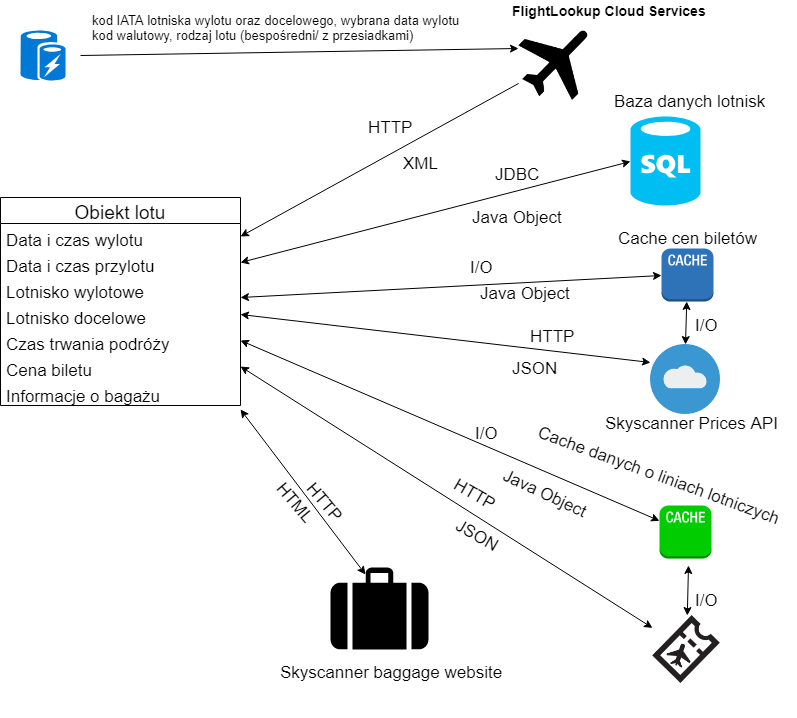
\includegraphics[scale=0.50, keepaspectratio]{search_module.png}
\caption{Schemat architektoniczny modułu wyszukiwania lotów}
\label{fig:search_module}
\end{figure}

Na rysunku 3.5.1 przedstawiono schemat zaprojektowanego modułu wyszukiwania połączeń lotniczych. Zobrazowano na nim przebieg procesu wyszukiwania z uwzględnieniem źródeł danych, sposobów ich uzyskiwania oraz rodzajów odpowiedzi. Górny opis strzałek oznacza metodę zwrócenia się o dane, natomiast dolny opisuje rodzaj zwróconej treści. Wyszukiwanie rozpoczynało się od wysłania żądania z kontrolera serwerowego do omawianego modułu. Żądanie to musiało uwzględniać w sobie parametry wyszukiwania. Moduł swoją pracę rozpoczyna od pozyskania danych lotniczych z serwisu FlightLookup. Treść odpowiedzi stanowi większą część całego obiektu lotu który ma zostać zwrócony. Po otrzymaniu tych danych moduł zwraca się do lokalnej bazy danych o udostępnienie danych lotnisk podając przy tym ich unikalne kody IATA\footnote{International Air Transport Association}. Następnym krokiem jest pozyskanie ceny lotu. Czynność ta rozpoczyna się od sprawdzenia czy poszukiwana informacja nie znajduje się w cache'u. Jeśli takie dane są zwrócone, cache natychmiastowo zwraca odpowiedni zasób. Jeśli natomiast taka informacja nie jest dostępna, moduł zwraca się do serwisów firmy Skyscanner o udostępnienie cen na poszukiwany przelot. Analogiczna sytuacja dokonuje się w przypadku pozyskiwania danych o linii lotniczej obsługującej lot. Ostatnim etapem jest wyszukanie informacji o dozwolonym bagażu podczas lotu. Jest to zrealizowane przez zwrócenie się do strony internetowej aplikacji Skyscanner posiadającej aktualne dane. Jej adres został wspomniany w rozdziale drugim. Po zebraniu wszystkich poszukiwanych informacji oraz sparsowaniu ich, obiekt lotu zwracany jest przez moduł wyszukiwania do kontrolera a następnie do części klienckiej gdzie użytkownik może obejrzeć wyniki całego procesu wyszukiwania.
\section{Komunikacja między komponentami aplikacji}
Opisane we wcześniejszych podrozdziałach komponenty narzucały sposoby komunikacji między nimi. Każde z nich zostanie w tym podrozdziale stosownie przedstawione. 
\subsection{Protokół HTTP}
Protokół HTTP\footnote{Hypertext Transfer Protocol} to jeden z najpopularniejszych i powszechnie przyjętych protokołów aplikacji w świecie internetu. Jest to wspólny język między serwerami a klientami umożliwiający modernistyczną sieć. Od prostego początku jako pojedynczego słowa i ścieżki dokumentu stał się protokołem nie tylko dla przeglądarek internetowych ale praktycznie też dla każdego oprogramowania i aplikacji sprzętowych\cite{http}. Cechą protokołu HTTP jest pisanie i negocjowanie reprezentacji danych, co umożliwia budowę systemów niezależnych od przesyłanych danych.
 Początkowo protokół ten powstał z oznaczeniem wersji 0.9. Jest to obecnie dość stara wersja, używana jednak jeszcze przez niektóre serwery. HTTP 0.9 zostało podniesione do wersji 1.1 który jest najczęściej wykorzystywanym protokołem w internecie. Standard HTTP/1.1 rozwiązał wiele niejednoznaczności protokołu, które znaleziono we wcześniejszych wersjach i wdrożył szereg kluczowych optymalizacji wydajnościowych, dodatkowe mechanizmy buforowania oraz enkrypcję transferu. Jako odpowiedż na ciągle zwiekszajacą się liczbę urządzeń podłączonych do internetu oraz wymagnia wobec niego, w 2012 roku zainicjowano protokół HTTP/2. Głównym jego celem jest poprawa wydajności transportu i osiągnięcie zarówno mniejszych opóźnień i wyższej przepustowości.
\subsection{JDBC}
JDBC\footnote{Java Database Connectivity} to standardowy, niezależny od bazy danych interfejs do interakcji z dowolnym źródłem danych opartym na tabelaryczności. Przeważnie jest używany do współdziałania z relacyjnym systemem zarządzania bazami danych. Za pomocą tego interfejsu można też korzystać z dowolnego tabelarycznego źródła danych, takiego jak arkusz csv, plik tekstowy itd. Zazwyczaj używa się go do łączenia z bazą danych, wyszukiwania danych i ich aktualizowania. Umożliwia także wykonywanie procedur SQL w bazie danych przy użyciu składni niezależnej od bazy danych.\cite{jdbc} Używanie JDBC zwalnia użytkownika z konieczności uczenia się nowej składni za każdym razem pracy na innej bazie danych. JDBC dostarcza zestaw oprogramowania w języku Java do przetwarzania zestawu wyników zapytań SQL w sposób niezależny od bazy danych. W opracowanej aplikacji interfejs JDBC pośredniczył pomiędzy relacyjną bazą danych MySQL a częścią serwerową aplikacji.
\subsection{I/O}
Operacje zapisu oraz odczytu są podstawowymi częściami systemów operacyjnych wraz z językami programowania oraz ich bibliotekami. Prawie wszystkie programy komputerowe wykonują pewne operacje zapisu/odczytu inaczej zwanymi operacjami wejściowymi i wyjściowymi. W opracowanej aplikacji za wykonywanie tych operacji odpowiadał język Java która przez system operacyjny zwracała się do zasobów plikowych lub pamięci podręcznej. Operacje I/O dotyczą systemu plików, który jest elementarnym składnikiem każdego systemu operacyjnego. Zarządza on archiwizacją danych oraz ich późniejszym odzyskiwaniem. System plików przetrzymuje dane w plikach, które zaś są przechowywane w katalogach. Dostęp do plików oraz katalogów uzyskuje się przez zdefiniowanie ścieżek dostępu, które lokalizują obiektu systemu plików.\cite{i/o}

\newpage
\chapter{Implementacja}
Następstwem stworzenia projektu aplikacji jest implementacja oprogramowania zawartego w założeniach pracy dyplomowej. Zostanie ona szczegółowo opisana w tym rozdziale. Jego treść została stworzona na podstawie projektu aplikacji oraz zagadnień poruszonych w poprzednich rozdziałach. Stworzona aplikacja została podzielona według założonych wymagań opisanych na stronie trzeciej. Została podzielona na dwie logiczne części: stronę serwerową oraz kliencką. Opisano je ogólnie w poprzednim rozdziale, w tej części pracy skupiono się zagadnieniach związanych z implementacją powstałego oprogramowania.

\section{Oprogramowanie po stronie klienta}
Część kliencka to osobna aplikacja osadzona w przeglądarce internetowej. Został w niej stworzony graficzny interfejs użytkownika oraz serwis odbierający dane od części serwerowej.
\subsection{Podział strukturalny}
Aplikacja kliencka została logicznie podzielona na cztery pakiety: 

\begin{figure}[!ht]
\centering
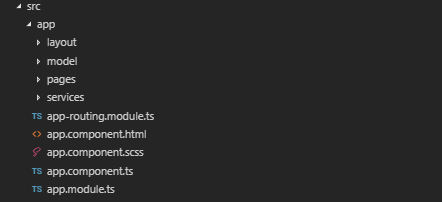
\includegraphics[scale=1.0, keepaspectratio]{client_structure.png}
\caption{Struktura plików części klienckiej}
\label{fig:client_structuresearch_module}
\end{figure}
\noindent Pakiet \textit{layout} przechowuje komponenty o wielokrotnym użyciu w aplikacji klienckiej. Katalog \textit{model} zawiera odpowiedniki klas modelowych z części serwerowej. Kolejnym elementem jest pakiet \textit{pages}. Znajdują się w nim komponenty renderujące kompletne strony internetowe. Zostały zbudowane z segmentów stworzonych w katalogu \textit{layout}. Ostatnią częścią aplikacji klienckiej jest pakiet \textit{services}. Zawiera on oprogramowanie odpowiedzialne za komunikowanie się z serwerem. 
\newpage
\subsection{Moduły pobierania danych}
W części klienckiej zaimplementowano serwisy odbierające dane z części serwerowej. Pierwszym z nich jest odpowiedzialny za połączenie z modułem wyszukiwania po stronie serwera. Zawiera on dane adresu sieciowego serwera udostępniającego zebrane wyniki wyszukiwania połączeń lotniczych.
\begin{lstlisting}[language=JavaScript, caption= Kod źródłowy funkcji pobierającej wyniki z serwera]
import { Injectable } from '@angular/core';
import { baseUrl } from '../../../environments/environment';
import { HttpClient } from '@angular/common/http';
import { Observable } from 'rxjs';
import { MultiFlight } from 'src/app/model/interfaces/MultiFlight';

@Injectable({
  providedIn: 'root'
})
export class FlightsService {

  getFlightsURL: string = baseUrl + 'api/flights/';

  constructor(private http: HttpClient) {
  }

  getFlights(originAirport: string, destinationAirport: string, departureDate: string, typeOfConnection: string, currency: string) : Observable<MultiFlight[]>{
    var requestUrl = this.getFlightsURL + originAirport + '/' + destinationAirport + '/' + departureDate + '/' + typeOfConnection + '/' + currency;
    return this.http.get<MultiFlight[]>(requestUrl);   
  }

}
\end{lstlisting}
Na powyższym listingu przedstawiono fragment oprogramowania pobierający wyniki wyszukiwania. Funkcja \textit{getFlights} przyjmuje 5 parametrów które dostarcza jej użytkownik. Pierwszym procesem tej funkcji jest zbudowanie adresu URL który posłuży do zbudowania żądania pobrania danych. Jej działanie polega na złączeniu wcześniej wspomnianych parametrów oddzielając je znakiem "/" w roli separatora. Ostatnim krokiem jest stworzenia żądania GET protokołu HTTP.

Drugim zaimplementowanym serwisem jest prosta funkcja pobierające dane o lotniskach. Jej działanie zostanie przedstawione na kolejnym listingu.
\begin{lstlisting}[language=JavaScript, caption= Kod źródłowy funkcji pobierającej dane lotnisk]
import { Injectable } from '@angular/core';
import { HttpClient, HttpErrorResponse } from '@angular/common/http';
import { baseUrl } from '../../../environments/environment';
import { Airport } from '../../model/interfaces/Airport';
import { Observable, throwError } from 'rxjs';
import { catchError, retry } from 'rxjs/operators';

@Injectable({
  providedIn: 'root'
})
export class AirportsService {

  getAirportsUsingIncompletePhraseURL: string = baseUrl + 'api/airports/getAirportsStartingWith/';

  getAirportsStartingWithPhrase(phrase: string): Observable<Airport[]>{
    return this.http.get<Airport[]>(this.getAirportsUsingIncompletePhraseURL + phrase).pipe(catchError(this.handleError)); 
  }  
}
\end{lstlisting}
Działanie przedstawionego kodu źródłowego rozpoczyna się od stworzenia adresu URL pod którym część serwerowa udostępnia poszukiwane dane. Do zmiennej \textit{baseUrl} oznaczającej domenę serwera zostaje dodana część sparametryzowana dla danych o lotniskach. Funkcja zwraca obiekty typu \textit{Airport} oraz dodatkowo obsługuje błędy zwrócone z drugiej części aplikacji.
\subsection{Interfejs graficzny}
Walory szybkości oraz użyteczności aplikacji tracą na znaczeniu jeśli budowane oprogramowanie nie jest wyposażone w czytelny interfejs użytkownika. Jest on formą interakcji pomiędzy użytkownikiem a aplikacją. Stworzone środowisko graficzne jest grupą wzajemnie współpracujących przycisków oraz obrazów zapewniających podstawowe poruszanie się po aplikacji klienckiej w obrębie przeglądarki internetowej. 
W części klienckiej zaimplementowano responsywny wygląd z takimi komponentami jak panel wyszukiwania lotów czy panel podróży wieloetapowej. Ich ogólny kształt i funkcje zostały w części zaczerpnięte z rozwiązań rynkowych aby zwiększyć konkurencyjność aplikacji klienckiej. 
\newpage
W bieżącym podrozdziale zostanie przedstawiony stworzony interfejs aplikacji wraz z krótkim opisem.

\begin{figure}[!ht]
\centering
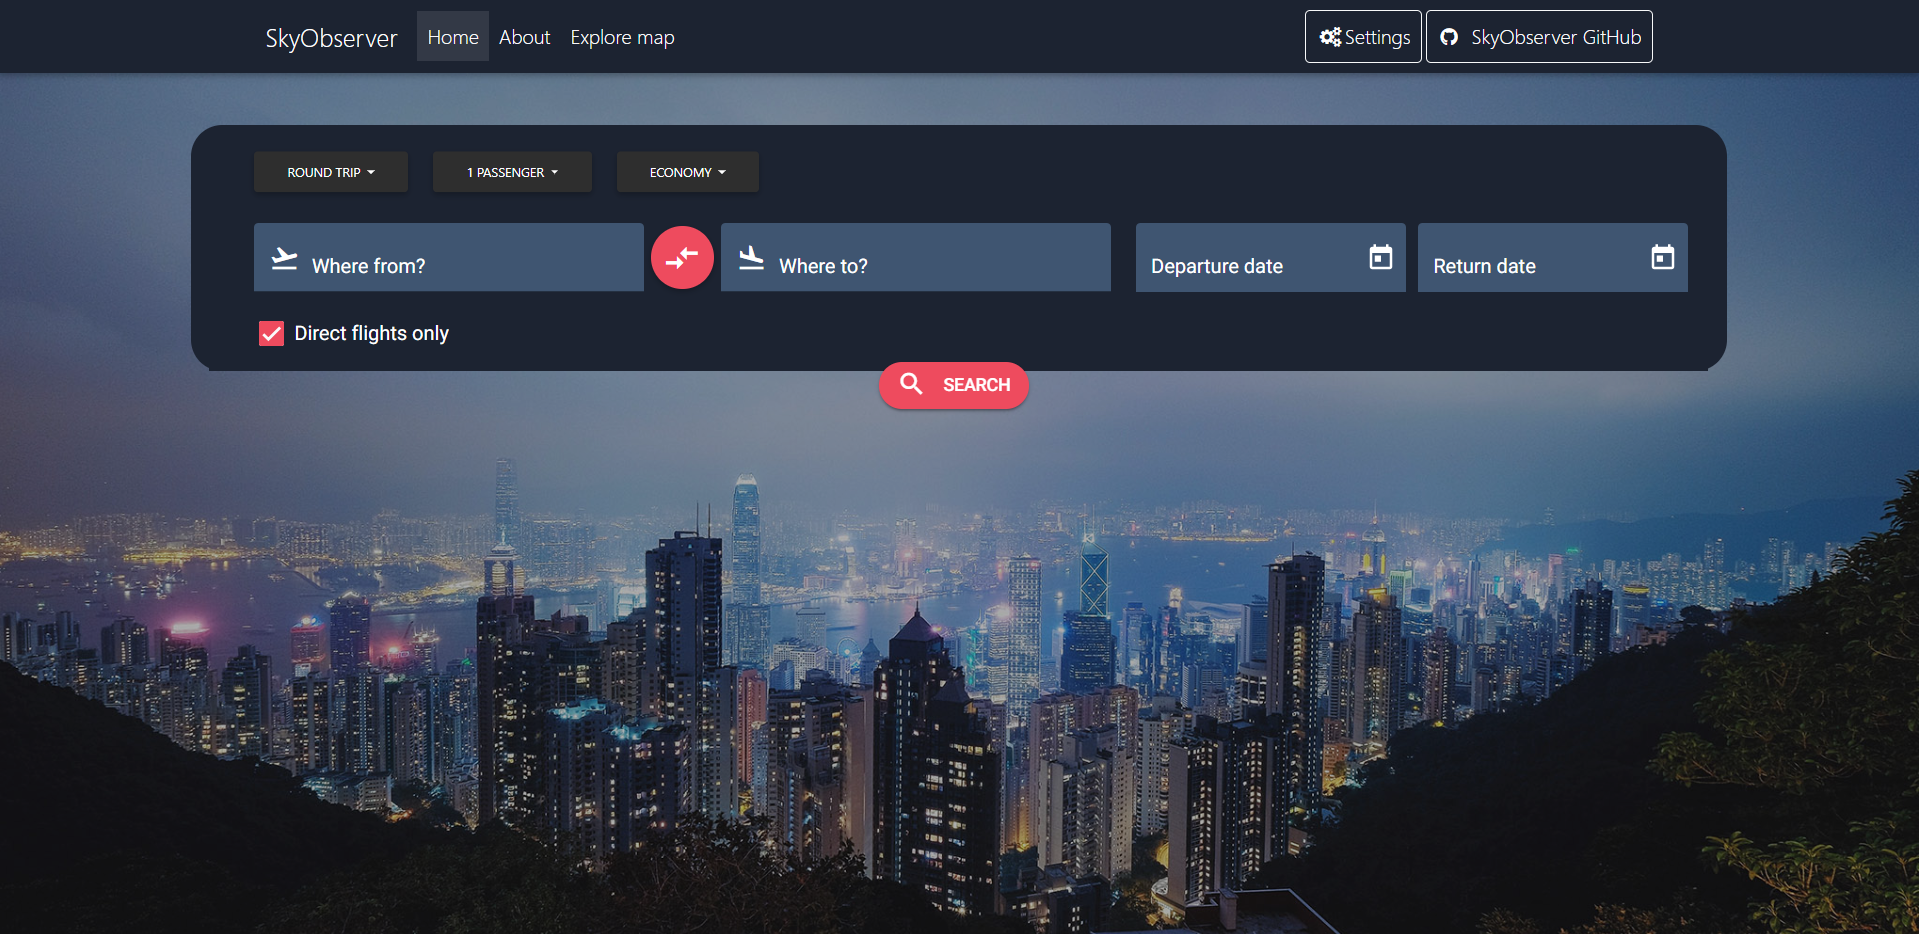
\includegraphics[scale=0.32, keepaspectratio]{client_main_page.png}
\caption{Strona główna aplikacji klienckiej}
\label{fig:client_main_page}
\end{figure}
Rysunek 4.1.2 przedstawia stronę startową części klienckiej. Jego tło jest na całej szerokości oraz długości wypełnione obrazem miasta Hongkong. Górna część strony przedstawia pasek nawigacyjny aplikacji, panel ustawień oraz odwołanie do repozytorium kodu stworzonej pracy dyplomowej. Następnym komponentem aplikacji klienckiej jest panel wyszukiwania lotów.

\begin{figure}[!ht]
\centering
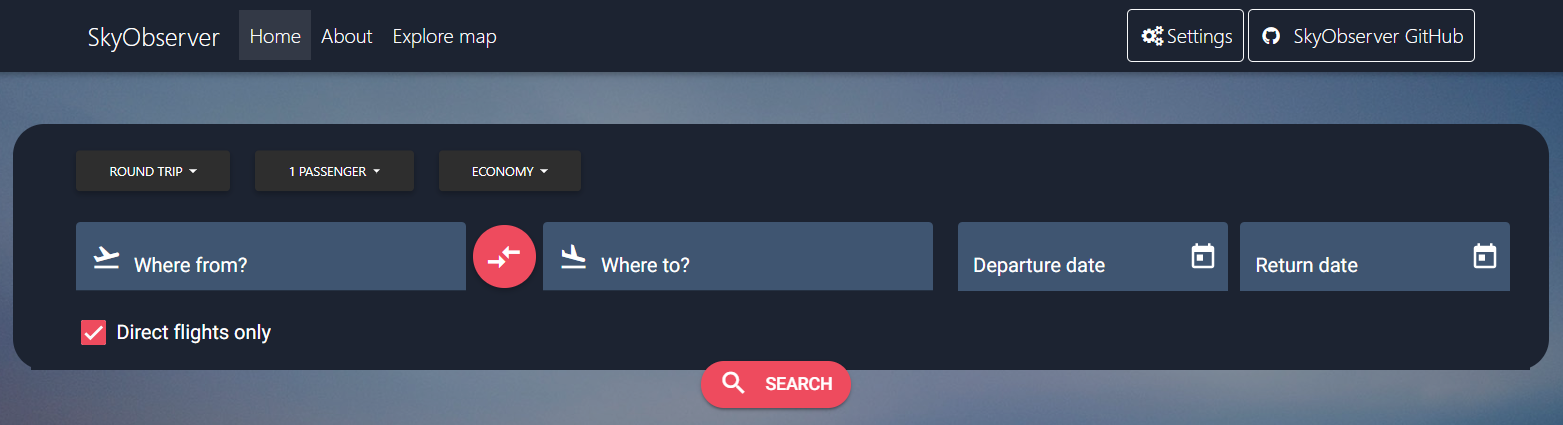
\includegraphics[scale=0.39, keepaspectratio]{search_panel.png}
\caption{Panel wyszukiwania połączeń lotniczych}
\label{fig:search_panel}
\end{figure}

Przedstawiony komponent obrazuje rozmieszczenie przycisków, pól wyboru parametrów wyszukiwania oraz dostępne opcje konfiguracyjne. Górna część panelu zawiera trzy przyciski konfiguracyjne. Odpowiadają one kolejna za wybór rodzaju lotu, ilość pasażerów oraz klasę poszukiwanego biletu lotniczego. W aplikacji założono trzy typy lotów: lot z możliwością powrotu, lot bezpośredni oraz podróż wieloetapową. Kolejna część poniżej opisanych przycisków przedstawia pola do wyboru parametrów poszukiwania. Ich ilość zmienia się w zależności od wybranego typu lotu.
\newpage
W elementach wyboru lotnisk został zaimplementowany mechanizm podpowiedzi wyszukiwania. Użytkownik po wpisaniu kilku pierwszych liter poszukiwanego miasta będzie mógł zobaczyć listę proponowanych lotnisk w obrębie tej miejscowości. 

\begin{figure}[!ht]
\centering
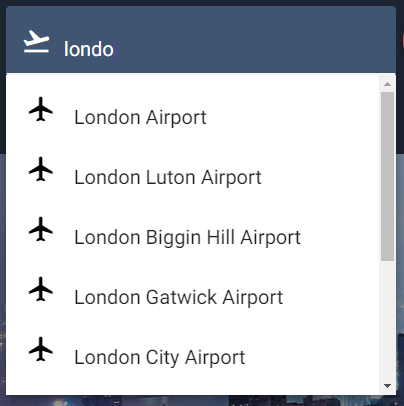
\includegraphics[scale=0.8, keepaspectratio]{airport_choose.png}
\caption{Komponent wyboru lotniska}
\label{fig:search_panel}
\end{figure}

Operacja ta jest dokonywana poprzez pobranie wpisanych liter a następnie zgłoszenia żądania do części serwerowej, która zwraca wyniki z bazy danych. Implementacja tego mechanizmu znalazła się w poprzednim podrozdziale. Użytkownikowi wyświetlane są pełne nazwy lotnisk. Po wybraniu poszukiwanego miejsca widoczna jest nazwa miasta wraz z unikalnym kodem IATA identyfikującym lotnisko. Elementem pomiędzy polami dotyczącymi wyboru lotnisk jest przycisk zamiany pól. Jego funkcją jest zamiana informacji zawartych w polach miejsca odlotu oraz przylotu. Ostatnimi elementami są pola wyboru dat lotu docelowego oraz powrotnego. Obecność drugiego jest uzależniona od wybranego typu lotu. W przypadku gdy wyszukiwany jest tylko w jedną stronę jest on niewidoczny a szerokość pierwszego jest rozszerzona. Kliknięcie w ikonę kalendarza wyzwala okno modalne z jego powiększonym widokiem. Szarym okręgiem jest na nim zaznaczony dzień dzisiejszy. Po wybraniu, data zapisywana jest w pamięci aplikacji. Ten zabieg służy do zabezpieczenia sytuacji przy ewentualnym wyborze daty powrotu. W takiej sytuacji aplikacja wskaże zapisaną datę jako najwcześniejszą wartość przy wyborze daty lotu powrotnego. \\ \indent
Ważnym komponentem w który włożono dużo pracy jest moduł podróży wieloetapowej. Umożliwia on zaplanowanie podróży złożonej z maksymalnie pięciu lotów w jedną stronę.

\begin{figure}[!ht]
\centering
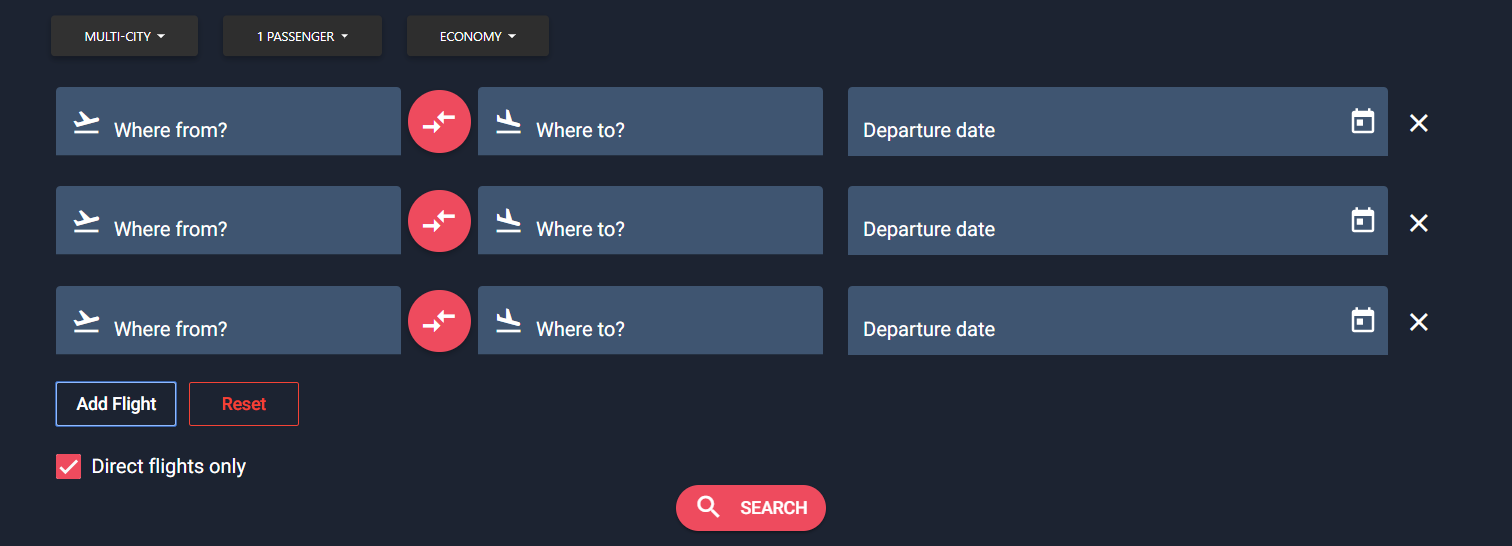
\includegraphics[scale=0.40, keepaspectratio]{multi_panel.png}
\caption{Komponent podróży wieloetapowej}
\label{fig:multi_panel}
\end{figure}
\noindent Rysunek 4.15 przedstawia wygląd opisywanego komponentu. Interfejs oferuje przyciski do dodawania kolejnych etapów podróży oraz ich usuwania. \\ \indent
Wspólnym elementem zarówno dla modułu wieloczęściowej podróży jak i podróży w jedną stronę i powrotnych jest przycisk wyszukiwania. Po kliknięciu go, aplikacja pobiera wprowadzone przez użytkownika parametry wyszukiwania i przekazuje je dalej do modułu odpytującego serwer. Moduł ten został przedstawiony w poprzednim podrozdziale. Wygląd przykładowych wyników wyszukiwania zaprezentowano na obrazku 4.1.6 Wyświetla on listę połączeń lotniczych pomiędzy wybranymi miejscami. Każdy element z tej listy jest rozwijalny, co oznacza że po kliknięciu na niego wysunie się dodatkowy obszar ze szczegółowymi informacjami o locie. W zależności od typu lotu wyświetlana jest zmienna liczba komponentów do wyboru połączenia lotniczego na wybranej trasie.
\begin{figure}[!ht]
\centering
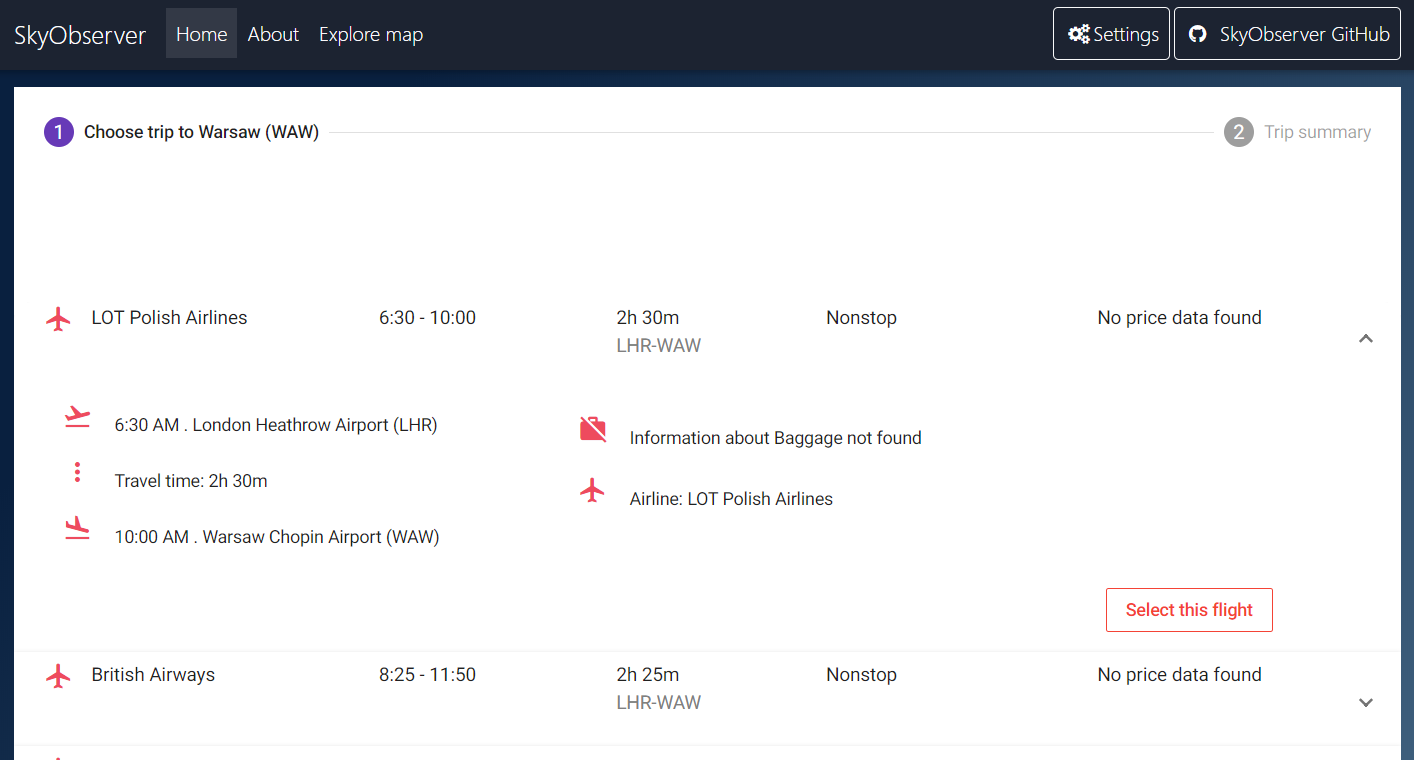
\includegraphics[scale=0.40, keepaspectratio]{result_component.png}
\caption{Wyniki wyszukiwania}
\label{fig:result_component}
\end{figure}


\newpage
\section{Oprogramowanie po stronie serwera}
Oprogramowanie serwerowe stanowi większą część całej aplikacji. Zostały w nim zaimplementowane mechanizmy parsowania, wyszukiwania i testowania danych lotniczych. Kwestie związane z użytymi technologiami przy tworzeniu serwera aplikacji zostały omówione w poprzednim rozdziale. W bieżącej części pracy zostanie opisana struktura części serwerowej, oprogramowanie odpowiedzialne za parsowanie różnych rodzajów danych jak i zaimplementowany moduł wyszukiwania.
\subsection{Struktura pakietowa}
Proces powstawania części serwerowej rozpoczął się od podzielenia tej części aplikacji na logiczne pakiety których nazwa związana byłaby z ich rolą. Poniższy rysunek prezentuje podział aplikacji.

\begin{figure}[!ht]
\centering
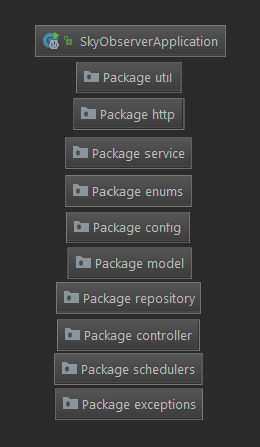
\includegraphics[scale=0.90, keepaspectratio]{server_structure.png}
\caption{Podział strukturalny części serwerowej}
\label{fig:server_structure}
\end{figure}

Omawianie tych katalogów najlepiej zacząć od pakietu \textit{config}. Jego zadaniem jest konfiguracja różnych parametrów serwera podczas jego startu. Ustawia on takie rzeczy jak klucze dostępowe do zasobów lotniczych, parametry lokalnego cache'u czy też zabezpieczenia aplikacji. Warstwa modelowa aplikacji znajduje się w pakiece \textit{model}. Zaimplementowane zostały w nim klasy modelowe które opisują obiekty krążące po całej aplikacji. Związanym z tym pakietem jest katalog \textit{repository}. Jest on miejscem na klasy implementujące pozyskiwanie obiektów odpowiadających klas modelowych. Niektóre z nich używają swoich analogicznych odpowiedników z pakietu \textit{service}. Potrzeba ta wynika z konieczności parsowania niektórych formatów danych do obiektów języka Java. Pakietem który udostępnia obiekty modelowe dla części klienckiej jest katalog \textit{controller}. Kod odpowiedzialny za wysyłanie żądań HTTP zaimplementowany jest w części \textit{http}. W części serwerowej zaimplementowano też moduły których wywołanie jest zaplanowane i precyzyjnie określone. Dotyczy to lokalnych plików przechowywujących dane o lotniskach oraz bagażach. Kod odpowiedzialny za ich aktualizowanie jest opracowany w katalogu \textit{schedulers}. Pozostałe pakiety \textit{util,enums} oraz \textit{exceptions} wprowadzają mniej znaczące dla aplikacji funkcje.  

\subsection{Oprogramowanie wyszukujące połączenia lotnicze}
Moduł wyszukiwania połączeń lotniczych został już opisany w poprzednim rozdziale, bieżący zostanie poświęcony kwestiom jego implementacji. Na potrzeby jego stworzenia opracowano specjalny sposób tworzenia obiektu lotu. Standardowy proces powstawania obiektu przez konstruktor języka Java okazał się mało czytelny dla wielu obiektów wchodzących w skład jednostki połączenia lotniczego. Dla tego obiektu opracowano implementację wzorując się na wzoru projektowym o nazwie \textit{Budowniczy}. Budowniczy to programistyczny wzorzec projektowy, który opisuje algorytm tworzenia złożonego obiektu z innych. Algorytm ten powinien być niezależny od składowych obiektu. Ponadto proces budowania powinien zezwalać na budowę różnych form tworzonego obiektu.\cite{builder}
Klasa modelowa \textit{Flight} została wyposażona klasę wewnętrzną ją budującą.Jej implementacja została przedstawiona na listingu 4.2.1
\begin{lstlisting}[language=java, caption=Fragment klasy Flight]
@JsonSerialize
public class Flight {
    private String departureTime;
    private String arrivalTime;
    private Airport originAirport;
    private Airport destinationAirport;
    private String duration;
    private CachedPrice price;
    private Airline airline;
    private Baggage baggage;
    
    ...
}
\end{lstlisting}
 \noindent Klasą odpowiedzialną za zbieranie danych o połączeniach lotniczych jest plik \textit{FlightsRepository}. W jej kodzie źródłowym zaimportowano wszystkie pozostałe repozytoria danych. Jego działanie polega na ustawieniu każdej jego składowej widocznej na listingu 4.2.2 pobierając odpowiednie dane z analogicznych repozytoriów tych składowych. Ze względu na złożoność oraz wielkość jego implementacji jego kod nie zostanie pokazany w tym rozdziale.

\subsection{Parsowanie danych}
Podrozdział ten jest odwołaniem do swojego odpowiednika w rozdziale trzecim. Zostanie w nim zwrócona szczególna uwaga na implementacje komponentów odpowiedzialnych za parsowanie różnych rodzajów danych.\\ \noindent
Opracowane następujące klasy parsujące:
\begin{itemize}[noitemsep,topsep=0pt]
\item AirlineParser - parser danych o liniach lotniczych konwertujący obiekty JSON na obiekty Java
\item AirportsParser - komponent pozyskujące obiekty z plików CSV
\item BaggagesParser - moduł parsujący dokumenty HTML
\item PricesParser - klasa konwertująca obiekty JSON dotyczące cen lotów
\item FlightsParser - moduł parsujący złożone treści otrzymane w języku znaczników XML na analogiczne obiekty języka Java
\end{itemize}
Wymienione komponenty zostaną krótko opisane wraz z przedstawieniem ich implementacji.
Ze względu na prostą złożoność jako pierwszy zostanie opisany parser danych linii lotniczych.
\begin{lstlisting}[language=java, caption=Implementacja parsowania treści JSON]
public class AirlineParser {
    private static final int FIRST_ELEMENT = 0;
    private Gson gson = new Gson();

    public Airline getAirlineObjectFromJSONResponse(String jsonObject) {
         Airline[] airlines = gson.fromJson(jsonObject, Airline[].class);
         return airlines[FIRST_ELEMENT];
    }
}
\end{lstlisting}
Powyższy listing przedstawia sposób konwersji treści w formacie JSON. Do tego celu posłużono się biblioteka gson firmy Google. Wywołując metodę \textit{fromJson} na obiekcie typu \textit{Gson} w prosty sposób odbywa się konwersja obiektów Json na obiekty \textit{Airline}. Funkcja jako wynik zwraca pierwszy element zparsowanej tablicy danych.\\ \indent
Translacja treści zwróconej z serwisu \textit{Flight Lookup} otrzymanej w postaci XML odbywała się przy pomocy biblioteki Jackson. Pierwszym krokiem było stworzenie odpowiedników elementów odpowiedzi na klasy modelowe w części serwerowej. Po tej czynności można było przystąpić do implementacji metody konwertującej.
\begin{lstlisting}[language=java, caption=Implementacja parsowania treści XML]
public class FlightsParser {
    private JacksonXmlModule xmlModule = new JacksonXmlModule();

    public OTA_AirDetailsRS getDeserializedXML(String XML) throws IOException {
        xmlModule.setDefaultUseWrapper(false);
        ObjectMapper objectMapper = new XmlMapper(xmlModule);
        return objectMapper.readValue(XML, OTA_AirDetailsRS.class);
    }
}

\end{lstlisting}
Powyższa implementacja jest podobna do poprzedniej przedstawionej na listingu 4.2.3 Metoda jako argument przyjmuje ciąg znaków XML. Do konwersji używana jest klasa \textit{ObjectMapper} pochodząca ze wcześniej wspomnianej biblioteki Jackson. Wynikiem zwróconym przez funkcję jest pojedynczy obiekt \textit{OTAAirDetailsRS} zawierający w sobie listę wszystkich wyszukanych lotów.
Ze względu na złożoność kodu źródłowego pozostałych parserów ich implementacja nie zostanie przedstawiona. Kod ten można znaleźć w dołączonym repozytorium, w pakiecie \textit{service}.
\newpage
\subsection{Kontrolery serwera}
W części serwerowej stworzono specjalny komponent odpowiedzialny za obsługę żądań wyszukiwania lotów oraz zwrócenie im poszukiwanych wyników. 
\begin{lstlisting}[language=java, caption=Implementacja parsowania treści XML]
@RestController
@RequestMapping("/flights")
public class FlightsController {

    @Autowired
    private MultiFlightsRepository multiFlightsRepository;
    private static final Logger logger = LoggerFactory.getLogger(PricesRepository.class);

    @GetMapping(value = "/{from}/{to}/{date}/{connection}/{currency}", produces = MediaType.APPLICATION_JSON_VALUE)
    public Collection<MultiFlight> searchForFlights(@PathVariable String from, @PathVariable String to, @PathVariable String date, @PathVariable String connection, @PathVariable String currency) throws AirportsNotFoundException, IOException {
        Collection<MultiFlight> flights = multiFlightsRepository.searchForMultiFlights(from, to, date, connection, currency);
        if (flights.isEmpty()){
            throw new FlightsNotFoundException();
        }
        return flights;
    }
}
\end{lstlisting}
Powyższy kontroler został zaimplemetnowany w pakiecie \textit{controller}. Dwie adnotacje nad deklaracją klasy tworzą w serwerze specjalne miejsce, w którym po podaniu odpowiednich parametrów kontroler zostanie wywołany. Parametry te opisane są nad deklaracją metody \textit{searchForFlights}. Funkcja pobiera z adresu URL kody IATA lotniska wylotowego oraz docelowego, datę wylotu, typ połączenia i kod walutowy. Przedstawione parametry są przekazywane w wywołaniu klasy repozytorium lotów, które zwraca wyniki wyszukiwania w postaci kolekcji obiektów. W przypadku nie znalezienia żadnych połączeń lotniczych, metoda zwraca wyrzuca wyjątek, który implikuje zwróceniem odpowiedzi o kodzie 404.
\chapter{Testy}
Proces powstawania oprogramowania jest zbiorem czynności opartych na wielu czynnikach. Patrząc wstecz, programowanie jako fach ma jedynie kilka dekad. Tworzenie oprogramowania można potraktować jako proces ewolucyjny gdzie ewoluuje ono z upływem czasu. Programiści szybko dochodzą do wniosków, że pisanie kodu jest trudne i podatne na liczne błędy. Wiele projektów zawodzi, ponieważ zespoły napotykają trudności ze złożonością tworzonych systemów. W wyniku tych niedociągnięć projekt nie zostaje skończony w terminie a koszt jego finalizacji przekracza początkowe oczekiwania\cite{testing}. Rozwój oparty na sprzężonym testowaniu tworzonego kodu jest jedną z praktyk efektywnego rozwoju oprogramowania. Testy potwierdzają funkcje aplikacji oraz jej użyteczność dla użytkownika. Standardowy podział ze względu na przeznaczenie można przedstawić następująco:
\begin{itemize}[noitemsep,topsep=0pt]
\item testy jednostkowe - potwierdzają poprawne działanie najmniejszych elementów systemu takich jak metody czy funkcje
\item testy integracyjne - sprawdzają poprawność integracji tworzonego oprogramowania z zewnętrznymi systemami
\item testy akceptacyjne - zapewniają o spełnieniu oczekiwań klienta który zamówił oprogramowanie
\item testy regresyjne - potwierdzają brak wpływu napisanego oprogramowania na pozostałe elementy systemu
\end{itemize}
W stworzonej aplikacji zdecydowano się na przetestowanie kluczowych fragmentów oprogramowania odpowiedzialnych za podstawowe funkcje systemu. Testy zaimplementowane zostały przy użyciu frameworków JUnit oraz Spring. Biblioteka JUnit to zewnętrzny pakiet oprogramowania dostarczająca zestaw narzędzi do testowania oprogramowania napisanego w języku Java. Znany i sprawdzony przez wielu programistów jest częścią wielu komercyjnych systemów. Drugi z nich, przedstawiony wcześniej w rozdziale trzecim dostarcza instrumenty do testowania jego oprogramowania serwerowego. \\ \indent
Podstawową metodą testującą oprogramowanie była asercja. Jest to predykat, który zwraca wartość logiczną. Najczęściej przyjmuje dwa argumenty a następnie porównuje je zwracając wynik\cite{assertion}. Napisane testy znajdują się w części serwerowej aplikacji, testują one poprawność odpowiedzi serwera, informacje otrzymane z zewnętrznych serwisów, parsowanie różnych formatów danych jak i najbardziej podstawowe elementy aplikacji. Nazwy testów przemawiają za kodem źródłowym który testują. Dla przykładu test dla klasy \textit{FlightRepository} będzie nazywał się \textit{FlightsRepositoryTest}. \\
\subsection{Testy jednostkowe}
Podstawowymi testami były testy jednostkowe. Na poniższym listingu przedstawiono zaimplementowany kod testujący poprawność działania funkcji zwracającej adres żądania HTTP.
\begin{lstlisting}[language=java, caption=Przykładowy test jednostkowy]
@Test
public void shouldReturnValidCacheKey() {
  assertEquals("WAW/LHR/20190110/DIRECT/PLN",
    multiFlightsRepository.buildCacheKey("WAW", "LHR", "20190110", "DIRECT", "PLN"));
    }
\end{lstlisting}
Bardziej złożonym przypadkiem jest test odpowiedzialny za sprawdzenie poprawnej ceny całej podróży.
\begin{lstlisting}[language=java, caption=Przykładowy test jednostkowy]
@Test
public void shouldReturnProperSumOfTotalFlightPrice() {
  Flight firstFlight = new Flight.Builder()
         .setPrice(new CachedPrice(200.43))
         .build();
 
  Flight secondFlight = new Flight.Builder()
         .setPrice(new CachedPrice(800.99))
         .build();

  Flight thirdFlight = new Flight.Builder()
         .setPrice(new CachedPrice(436.67))
         .build();
  List<Flight> flightList = List.of(firstFlight, secondFlight, thirdFlight);
  assertEquals(1438.09, multiFlightsRepository.calculateTotalFlightPrice(flightList), 0.001);
    }
\end{lstlisting}
Test zaprezentowany na listingu 5.0.2 inicjalizuje 3 obiekty typu \textit{Flight} z podanymi "na sztywno" wartościami cen przelotów. Obiekty te łączone są w kolekcję. Końcowa asercja sprawdza poprawbedziałanie metody \textit{calculateTotalFlightPrice} porównując jej wynik z oczekiwaną wartością. Warto zwrócić na trzeci argument jaki przyjmuje metoda \textit{assertEquals}. Oznacza on dopuszczalną różnicę między oczekiwanym a otrzymanym wynikiem.
\newpage
\subsection{Testy integracyjne}
Specyfikacja projektu narzucała konieczność przetestowania integracji napisanego oprogramowania z zewnętrznymi systemami. Testowano poprawność pobierania danych oraz ich oczekiwane parametry. Wszystkie klasy z pakietu \textit{repository} zostały przetestowane w sposób analogiczny do siebie.
\begin{lstlisting}[language=java, caption=Przykładowy test jednostkowy]
@Test
public void shouldReturnProprtAirlineObjectFromAPI() throws IOException {
     Airline airline = airlineRepository.getAirlineFromApi("AA");
     assertEquals(airline.getNameAirline(), "American Airlines");
     assertEquals(airline.getStatusAirline(), "active");
     assertEquals(airline.getCallsign(), "AMERICAN");
     assertEquals(airline.getNameCountry(), "United States");
    }
\end{lstlisting}
Oprogramowanie przedstawione na listingu powyżej testuje funkcjonowanie repozytorium zwracające informacje o liniach lotniczych. W pierwszym kroku pobiera ono obiekt linii lotniczej. Po przypisaniu tych danych do obiektu, sprawdzane są poszczególne parametry zwróconych informacji. \\ \indent
Test o analogicznej funkcji sprawdzał też repozytorium zwracające ceny lotów.
\begin{lstlisting}[language=java, caption=Przykładowy test jednostkowy]
@Test
public void shouldReturnValidPriceObject() throws IOException {
  CachedPrice price = pricesRepository.getFlightPrice("PLN", "WAW", "LHR", "20190128", "20190130");
  assertNotNull(price);
  assertEquals(price.getCurrency(), "PLN");
  assertEquals(price.getOriginPointOfRoute(), "WAW");
  assertEquals(price.getDestinationPointOfRoute(), "LHR");
}
\end{lstlisting}

\newpage
\chapter{Uwagi i wnioski}
Opracowanie aplikacji wyszukującej połączenia lotnicze było zadaniem trudnym i wymagającym bardzo dużej ilości pracy. Droga do stworzenia oprogramowania spełniającego wszystkie wymagania przedstawione w celach pracy wymagała głębokiego zrozumienia logiki biznesowej związanej z danymi lotniczymi. Do największych wyzwań podczas pracy z pewnością należało znalezienie odpowiednich źródeł danych udostępniających dane o lotach. Wysłano szereg zgłoszeń mailowych z prośbą o udostępnienie takich danych. W większości przypadków odpowiedzi były negatywne lub niesatysfakcjonujące z powodu żądania od dostawcy pokaźnej zapłaty za korzystanie z usługi. W warunkach akademickich skorzystanie z takich rozwiązań było niemożliwe. Po wnikliwej analizie rynku danych lotniczych udało się znaleźć odpowiednie źródło informacji dla potrzeb stworzonej aplikacji. \\ \indent
 Z dużą dozą pewności można stwierdzić iż opracowana aplikacja w pełni spełnia założone wymagania. Pozwala z całkiem dobrą szybkością wyszukiwać połączenia lotnicze oraz dostarczać wielu dodatkowych informacji z nimi powiązanych. W sposób logiczny i przemyślany zaprojektowano moduł wyszukiwania lotów. Opracowano dla niego specjalną architekturę która została odzwierciedlona w kodzie źródłowym pod postacią wzorca projektowego. Dzięki temu zabiegowi aplikacja zachowuje potencjał łatwego i mało problemowego rozwoju. \\ \indent
Zaimplementowany system został wyposażony w bogaty interfejs użytkownika. Opracowany w nowoczesnej technologii Angular, poziomem dobrego stylu i wyglądu dorównuje komercyjnym aplikacjom internetowym. Część pomysłów na jego kreatywną realizację zaczerpnięto z obecnych wyszukiwarek na rynku. \\ \indent
Z uwagi na warunki akademickie aplikację można usprawnić na wielu płaszczyznach. W stworzonej pracy zabrakło takich dodatkowych funkcji jak możliwość wyszukiwania lotów również z pobliskich lotnisk od aktualnie wybranego czy też wprowadzenia wersji w języku polskim. Część serwerowa mogłaby zostać poprawiona w zakresie "czystości kodu" oraz poprawnego nazewnictwa jej elementów. Istotne znaczenie dla podniesienia atrakcyjności aplikacji byłoby też zwiększenie poziomu jej responsywności. Część kliencka wymaga w tym zakresie lekkich poprawek. \\ \indent
Stworzonej aplikacji internetowej nadano nazwę \textit{SkyObserver}\footnote{SkyObserver - obserwator nieba}. Jest ona zwieńczeniem zebranej wiedzy i doświadczenia podczas studiów inżynierskich. Praca nad nią zaowocowała pogłębieniem technicznego sposobu myślenia oraz zrozumieniem wyzwań XXI wieku stawianym inżynierom informatykom.























\begin{thebibliography}{9}
\bibitem{xml}
XML. Almanach, Elliotte Rusty Harold, W.Scott Means, Wydawnictwo O'REILLY

\bibitem{json}
  \url{https://www.json.org/} \\
  Stan na dzień 03.01.2019

\bibitem{html}
	\url{https://en.wikipedia.org/wiki/HTML} \\
	Stan na dzień 04.01.2019
\bibitem{ehcache}
Instant Effective Caching with Ehcache, Daniel Wind, Packt Publishing


\bibitem{architektura}
tworzenie architektury oprogramowania, Christine Hofmeister, Robert Nord, Wydawnictwo Naukowo-Techniczne Warszawa

\bibitem{uml}
	Diagramy UML | Michał Wolski\\ \url{https://www.michalwolski.pl/diagramy-uml} \\
	Stan na dzień 16.01.2019
	
\bibitem{mysql}
MySQL Darmowa baza danych - Ćwiczenia praktyczne, Marcin Lis, Wydawnictwo Helion

\bibitem{jvm}
Java Programming Basics, Simon Roberts, Addison-Wesley Professional

\bibitem{http}
HTTP Protocols, Ilya Grigorik, wydawnictwo O'REILLY

\bibitem{jdbc}
Beginning Java 8 APIs, Extensions and Libraries Swing, JavaFX, JavaScript, JDBC and Network Programming APIs, Altamash Shaikh

\bibitem{i/o}
Java I/O, NIO, NIO.2, Jeff Friesen

\bibitem{builder}
Design Patterns: Elements of Reusable Object-Oriented Software, John Vlissides, Ralph Johnson, Richard Helm, Erich Gamma

\bibitem{testing}
Java Unit Testing with JUnit 5, Shekhar Gulati, Rahul Sharma

\bibitem{assertion}
Asercja,Wikipedia \\
\url{https://pl.wikipedia.org/wiki/Asercja_(informatyka)} \\
Stan na dzień 14.01.2019

\end{thebibliography}
\end{document}